\chapter{Background and Theoretical Basis}

In this section, we present an overview of Particle Physics and Quantum Field Theory (QFT) upon which the work contained in this thesis depends. We begin by discussing the Standard Model (SM) of Particle Physics and how modern experiments at the Large Hadron Collider (LHC) test it. We then focus on Quantum Chromodynamics (QCD), which is the part of the SM that describes the interactions of quarks and gluons, the fundamental particles that come together to form protons, neutrons and a whole range of other composite particles \cite{PDG}. Finally, we delve into the Spinor Helicity formalism \cite{Elvang2013} to introduce notation and derive results that will allow for a simple and clear method of performing the work presented in the later chapters of this thesis. 

\section{The LHC and the Standard Model}

The SM, shown in figure \ref{fig:SM}, is currently our best theoretical model for understanding the fundamental particles of nature and their interactions. It is also one of the most rigorously tested models in the history of physics and to date it has stood up to all the tests thrown at it \cite{Ellis1995}. For instance, the measurement of the anomalous magnetic dipole moment of the electron agrees with that predicted by the model to ten significant figures \cite{Aoyama2012}. Despite these successes, however, we know that the SM cannot be a \emph{complete} model of our universe. For instance, it does not include gravity in its formulation. On top of that, cosmological measurements such as that of the velocities of spinning galaxies and the expansion rate of the universe imply that there is a whole other sector we are currently ignorant of: that of Dark Matter and Dark Energy \cite{Bertone2005}. Indeed, some estimates suggest that approximately 96\% of the universe consists of these mysterious quantities \cite{Jarosik2011}. Clearly, we need to find a way forward in order to develop a theory `Beyond the Standard Model' that can describe them. One possibility is that non-SM particles could interact with SM particles in a manner whereby we would need to be able to calculate SM predictions to a large degree of precision to be able to determine if they are there \todo{reword 'one poss' sentence as it is clumpy}. Theorists and experimentalists must continue to come together in order to face this challenge; theorists by improving how calculations are conducted and experimentalists by reducing experimental uncertainties and collecting ever more data. \\

\begin{figure}[t]
\centering
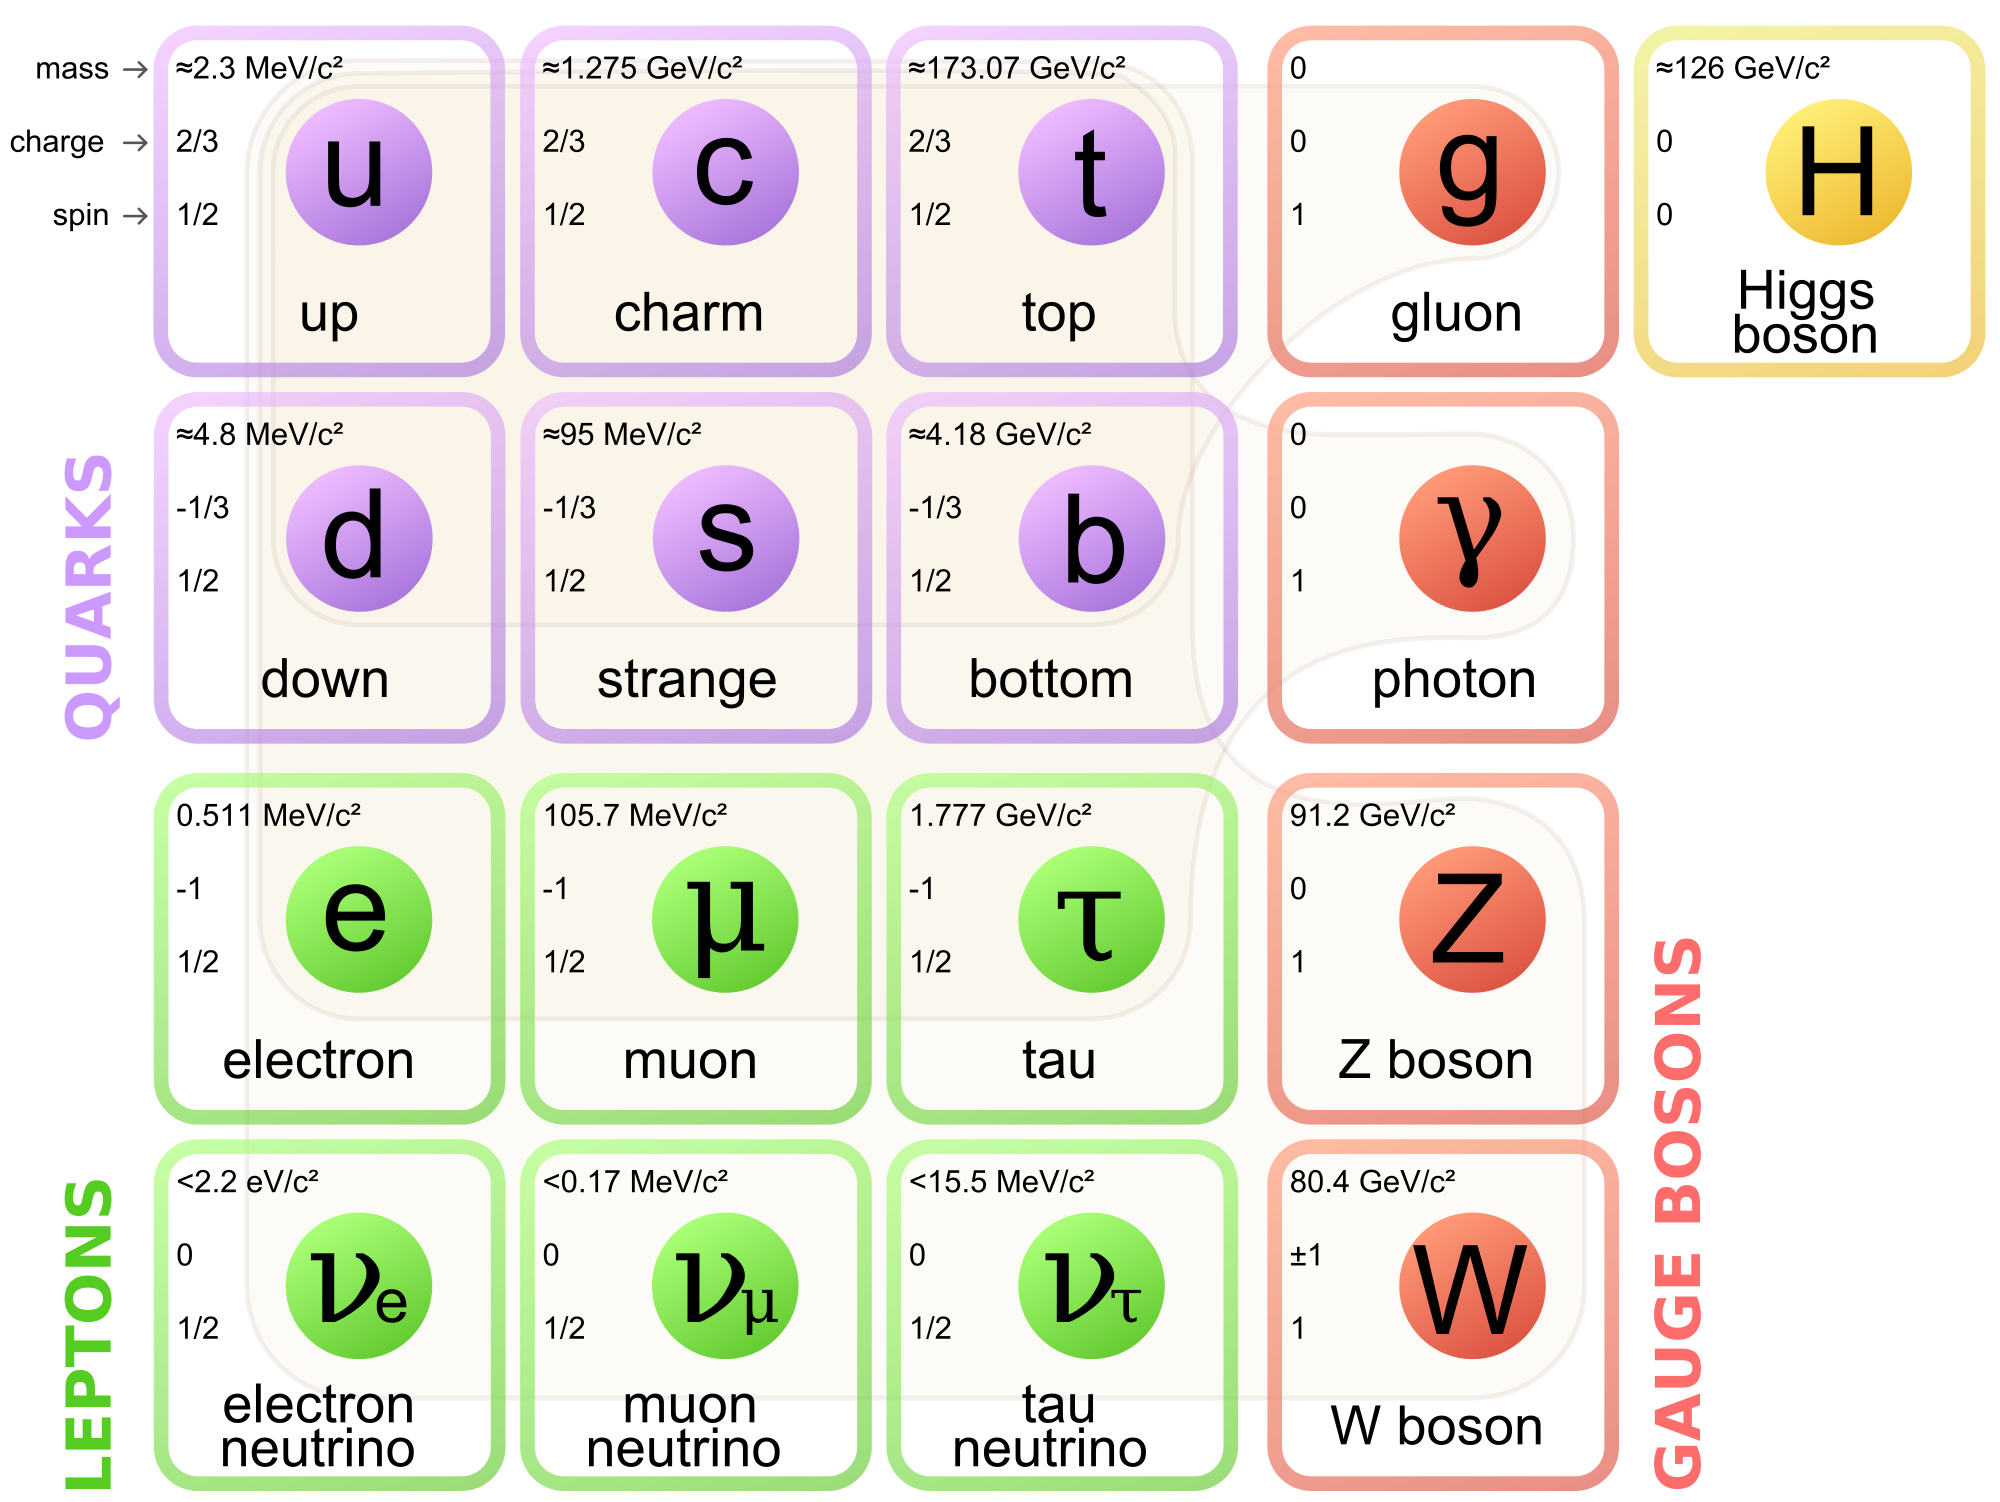
\includegraphics[scale=0.2]{Images/SM.png} 
\caption{The Standard Model of Particle Physics. Image from the Wikipedia page on the Standard Model.}
\label{fig:SM}
\end{figure}

%The SM is split into two parts; quarks and leptons which are the actual particles that make up larger structures such as atoms and gauge bosons that allow for the particles to interact with each other via forces. \\
%\\
The LHC has given physicists the opportunity to probe the SM at the highest energies yet, ultimately being able to reach a centre-of-mass energy of 14 TeV. This is approximately 7 times higher than what was achievable at its spiritual predecessor, the Tevatron at Fermilab \cite{Holmes2011}. The headline story for the LHC, of course, was its discovery of the Higgs boson in 2012, the physical remnant of `Electroweak Symmetry Breaking' (EWSB) \cite{Aad2012,Higgs1964}. In effect, the masses of the fundamental particles are generated via interactions with the Higgs field, and so it is often said that the discovery of the Higgs is the discovery of the `origin of mass'. At this stage, we do not know whether the Higgs boson that has been discovered is exactly the one predicted by the Standard Model. Much more research now needs to be done in order to determine its fundamental properties, such as the strength of its coupling to the massive gauge bosons, before we can know one way or the other. This presents the very exciting theoretical challenge of providing accurate predictions for Higgs processes, and Chapter 4 of this thesis will explore this issue further. The theory that we will mostly concern ourselves with, however, is not that of EW physics but rather QCD. The following sections will provide an overview of the theory in order to discuss some important aspects and also to provide a basic introduction to QFT, which underpins the entirety of the SM. 

\section{QCD}

QCD is described by a non-Abelian $SU(3)$ gauge group within the SM and provides the theoretical underpinning for the \emph{strong interaction}, the interaction between \emph{quarks} and \emph{gluons}. This then confines our study to the purple area and the very top of the red area shown in figure \ref{fig:SM}. This may seem restrictive, but because the LHC collides protons which consist of quarks and gluons, it is clearly QCD that is the underlying theory we need to use to understand the collisions that happen there. 

\subsection{Lagrangian Formalism and Dirac Fermions}
QFTs have their foundations in Lagrangian mechanics and so we will here review the background of the formalism. The fundamental quantity is the \emph{action}, the time integral of the Lagrangian $L$:

\begin{equation}
S = \int L \hspace{2pt} dt.
\end{equation}

In a local field theory, we can write the Lagrangian as a integral over all space of the \emph{Lagrangian Density}, $\mathscr{L}$, which can depend on a set of fields and the derivatives of those fields, $\mathscr{L} = \mathscr{L}(\phi_i, \partial_\mu \phi_i)$. From this point onwards, we will refer to the `Lagrangian density' as just the `Lagrangian'. We therefore have

\begin{equation}
S = \int \mathscr{L} (\phi_i, \partial_\mu \phi_i) \hspace{2pt} dt \hspace{2pt} d^3 x = \int \mathscr{L} (\phi_i, \partial_\mu \phi_i) \hspace{2pt} d^4 x,
\end{equation}

where we note that we work in units such that $c = \hbar = 1$. The \emph{principle of stationary action} states that as a system evolves from one configuration to another, it does so in a way that minimises the action; $\delta S = 0$. By considering a small change on the right-hand side of the previous equation, we arrive at the famous \emph{Euler-Lagrange} equations of motion,

\begin{equation}
\label{eqn:el}
\partial_\mu \left( \frac{\partial \mathscr{L}}{\partial (\partial_\mu \phi_i)} \right) - \frac{\partial \mathscr{L}}{\partial \phi_i} = 0.
\end{equation}

The field content of QCD consists of quarks and gluons, so they must be included in the Lagrangian in such a way that the appropriate equations of motion are recovered from it. We will begin with quarks. They are fermionic particles and so (when not interacting or, more simply, `free') will obey the Dirac equation

\begin{equation}
(i \slashed{\partial} - m) \psi(x) = 0,
\end{equation}

where $\slashed{\partial} \equiv \gamma^\mu \partial_\mu$ and $m$ is the mass of the quark. Suppressed here is the fact that this is actually a matrix equation in spinor space; $\psi$ is a four-component spinor and the $\gamma^\mu$ are a set of four-by-four matrices with the anti-commutation relation $\{\gamma^\mu, \gamma^\nu\} = 2 \eta^{\mu \nu}$. An explicit form for the matrices $\gamma^\mu$ will be presented later in the chapter since it is not necessary to have one at this point. We introduce a conjugate field $\bar{\psi}(x) = \psi^\dagger(x) \gamma^0$ and write a Lagrangian

\begin{equation}
\mathscr{L} = \bar{\psi}(x)(i \slashed{\partial} - m) \psi(x),
\end{equation}

where now we can evaluate the Euler-Lagrange equation with respect to the field $\bar{\phi}$ to yield the Dirac equation for $\psi$, as we wanted. The reason $\bar{\psi}$ is used as a conjugate field as opposed to the more obvious $\psi^\dagger$ comes from the requirement that the Lagrangian is invariant under a Lorentz transformation; in other words, $\mathscr{L}$ is a Lorentz scalar. We could also, of course, take the variation of this Lagrangian with respect to $\psi$ and doing so we get

\begin{equation}
\bar{\psi}(x)(i \slashed{\partial} + m) = 0,
\end{equation}

which is the Hermitian conjugate of the previous equation. The Dirac equation has plane wave solutions of the form

\begin{equation}
\label{eqn:dirac}
\psi(x) = u\left(\vec{p}\right )e^{- i \hspace{1pt}p \cdot x} + v\left(\vec{p}\right ) e^{i \hspace{1pt} p \cdot x},
\end{equation}

where $p$ is the four-momentum and $\vec{p}$ the three-momentum. In practice it is the $u$ and $v$ spinors that are used in calculations and they are interpreted as describing fermions and anti-fermions respectively. \\
\\
One of the great successes of the Dirac equation is that it predicts the existence of anti-fermions. Imagine that we are in a frame such that $\vec{p} = 0$. Since $p \cdot x = Et - \vec{p}\cdot \vec{x}$ and $E = \sqrt{\vec{p}^2 + m^2}$, then the second term in equation \ref{eqn:dirac} will have an exponential $e^{i m t}$ -- a state with negative energy\footnote{To be more precise, the sign of $i$ chosen in the Schr\"odinger equation is a matter of convention and so strictly speaking it is not just the sign of the exponential that determines that this is an anti-fermion. Rather, it is because we have \emph{both} plus and minus sign solutions and we are required to consider both of them.}. Because Quantum Mechanics requires a complete set of basis states, we cannot simply throw the solution away as `unphysical'. The solutions have to be interpreted as either positive energy fermions moving backwards in time or negative energy anti-fermions moving forwards in time. We will see later how the former interpretation lends itself rather neatly to a graphical representation of scattering involving fermionic particles. In any case, substituting this form for $\psi(x)$ into the Dirac equation, we find the following conditions:

\begin{subequations}
\begin{align}
(\slashed{p} - m)u(\vec{p}) &= 0, \\
(\slashed{p} + m)v(\vec{p}) &= 0.
\end{align}
\end{subequations}

%Put more spinor stuff here?

\subsection{Gauge Symmetry}

We briefly mentioned that QCD is a gauge theory with gauge group $SU(3)$. This is a non-abelian group, which we will see later leads to a whole host of interesting effects. For the time being, however, we will switch to the abelian group $U(1)$, which is the group describing Quantum Electrodynamics (QED), in order to make it easier to derive some results that we can still use for the more complicated group $SU(3)$. In either case, the symmetry we require in the Lagrangian is that it is unchanged if we redefine our charges according to a group transformation, $\psi \to U \psi$. For a global redefinition where our operator $U$ does not depend on $x$, this is trivially true since the $U$s are by definition unitary. However, if we generalise to a local redefinition,

\begin{equation}
\begin{split}
\mathscr{L}'& = \bar{\psi}(x)U^\dagger(x)(i \slashed{\partial} - m) U(x)\psi(x)\\
& = \bar{\psi}(x)(i \slashed{\partial} - m)\psi(x) + i \bar{\psi}(x) U^\dagger(x)\gamma^\mu\left[\partial_\mu U(x) \right]\psi(x) \neq \mathscr{L}.
\end{split}
\end{equation}

The problem has appeared because of the derivative in our Lagrangian. What we would like is a different derivative term that includes the partial derivative but along with an extra part to cancel away the extra term. Equivalently, we search for a so-called \emph{covariant derivative} that transforms as

\begin{equation}
D_\mu ' = U(x) D_\mu U^\dagger (x).
\end{equation}

Such an object can be constructed, but we have to introduce another field, $A_\mu$, that transforms non-trivially. Before we do so, however, let us take the specific example of the $U(1)$ group and explicitly evaluate the extra term. If we call the group generator $\Lambda$, then

\begin{equation}
U(x) = e^{i q \Lambda(x)},
\end{equation}

where $q$ is an overall scale factor, which is associated with the group charge. Then the extra term is proportional to

\begin{equation}
\partial_\mu U(x) = i q (\partial_\mu \Lambda(x)) e^{i q \Lambda(x)}.
\end{equation}

Let us define our covariant derivative in the following way:

\begin{equation}
\label{eqn:covder}
D_\mu = \partial_\mu + i q A_\mu(x).
\end{equation}

Then, under the gauge transformation:

\begin{equation}
\begin{split}
D_\mu' \psi'(x) & = (\partial_\mu + i q A_\mu'(x)) e^{i q \Lambda(x)} \psi(x) \\
& = U(x)(\partial_\mu + iq[A_\mu'(x) + (\partial_\mu \Lambda(x))])\psi(x),
\end{split}
\end{equation}

and therefore we can recover invariance so long as

\begin{equation}
A_\mu'(x) = A_\mu(x) - \partial_\mu \Lambda(x),
\end{equation}

which we recognise precisely as a gauge transformation of the vector potential $A^\mu$. The process of constructing a covariant derivative in this manner is called the \emph{principle of minimal coupling} and can be applied to any given gauge group. Thus, we simply replace the partial derivative in our Lagrangian with the covariant derivative to get a locally gauge invariant Lagrangian:

\begin{equation}
\begin{split}
\mathscr{L}_{Dirac+Interation} &= \bar{\psi}(x)(i \slashed{D} - m)\psi(x) \\
& = \bar{\psi}(x)(i \slashed{\partial} -m) \psi(x) + i q \bar{\psi}(x) \slashed{A}(x) \psi(x).
\end{split}
\end{equation}

From the requirement of local gauge invariance alone, we see from the second term that there is necessarily an interaction between the matter content and the gauge boson. However, our current form of the Lagrangian does not yet include a term that describes the dynamics of the gauge field itself. We know that such a term must be gauge and Lorentz invariant. Consider what would happen if we included a derivative of the field $A_\mu$ in our formalism and applied the gauge transformation;

\begin{equation}
\partial_\mu ' A_\nu'  (x) = \partial_\mu (A_\nu(x) - \partial_\nu \Lambda(x)).
\end{equation}

This is clearly not gauge invariant, but the combination anti-symmetric in $\mu,\nu$ is:

\begin{equation}
\begin{split}
\partial_\mu ' A_\nu' (x) - \partial_\nu' A_\mu'(x) & = \partial_\mu (A_\nu(x) - \partial_\nu \Lambda(x)) -  \partial_\nu (A_\mu(x) - \partial_\mu \Lambda(x)) \\
&= \partial_\mu A_\nu (x) - \partial_\nu A_\mu(x) \equiv F_{\mu \nu}, 
\end{split}
\end{equation}

where the last line follows from the fact that derivatives commute with each other. The object $F_{\mu \nu}$ is called the \emph{field strength tensor}. This can also be defined in the form

\begin{equation}
F_{\mu \nu} = -\left (\frac{i}{q} \right)[D_\mu, D_\nu],
\end{equation}

which is a form that will be useful when generalising to other gauge groups. The last requirement is to insert this into our Lagrangian in a Lorentz invariant fashion\footnote{Actually, we should really also include a term $\sim \epsilon^{\alpha \beta \mu \nu}F_{\alpha \beta} F_{\mu \nu}$ since this too is Lorentz invariant, but such a term is parity violating and this thesis will only concern itself only with theories that are parity-symmetric.} and also make explicit that there are potentially many fermions that can interact with the $U(1)$ gauge bosons in this way:

\begin{equation}
\mathscr{L}_{QED} = \sum_{f \hspace{1pt} \in \hspace{1pt} flavours} \bar{\psi}_f(x)(i \slashed{D} - m)\psi_f(x) - \frac{1}{4}F_{\mu \nu}F^{\mu \nu},
\end{equation}

where we have added an arbitrary normalisation factor to our new term for convenience. 

\subsection{QCD Lagrangian} 

The question of how to go from QED to QCD is equivalent to the question of what extra considerations need to be made if we work with the group $SU(3)$ rather than $U(1)$. The first difference is that $SU(3)$ has $3^2 - 1 = 8$ generators and so 8 independent rotation directions for our operator $U$. Thus, a (local) group transformation will have the form

\begin{equation}
U(x) = e^{i g_s \Lambda^a(x)t^a},
\end{equation}

where $t^a$ are the generators of the group. Additionally, in the fundamental representation of $SU(3)$, the Dirac spinors must be a 3-vector,

\begin{equation}
\psi = \begin{pmatrix}
    q^r \\
    q^b \\
    q^g
\end{pmatrix} ,
\end{equation}

where $q$ is a specific flavour of quark (the entire theory has all of them, of course) and $r,g,b$ are colour labels, denoting the SU(3) `colour' charge'. Now we apply the principle of minimal coupling from the previous section to find a covariant derivative for this gauge group, being explicit with our colour space notation:

\begin{equation}
D_\mu = \partial_\mu \mathbb{1} + i g_s t^a A^a_\mu(x).
\end{equation}

Each of the 8 gauge fields has to transform in the same way as before so as to make the covariant derivative perform its function correctly,
\begin{equation}
A_\mu^{a'} = A^a_\mu + \partial_\mu \Lambda^a(x),
\end{equation}

and the final step is to construct the field strength tensor

\begin{equation}
\begin{split}
F_{\mu \nu} &= -\left(\frac{i}{g_s}\right) [D_\mu, D_\nu] \\
& =-\left(\frac{i}{g_s}\right) [\partial_\mu + i g_s A_\mu^a t^a, \partial_\nu + i g_s A_\nu^b t^b] \\
&= [A_\mu^a t^a, \partial_\nu] + [\partial_\mu, A_\nu^b t^b] + i g_s A^a_\mu A_\nu^b[t^a, t^b] \\
&= A^a_\mu t^a \partial_\nu - (\partial_\nu A_\mu^a) t^a + (\partial_\mu A_\nu^b) t^b - A_\nu^b t^b \partial_\mu + i g_s A^a_\mu A_\nu^b [t^a, t^b] \\
&= t^c( \partial_\mu A_\nu^c - \partial_\nu A_\mu^c) + i g_s A_\mu^a A_\nu^b (i f^{abc}t^c) \\
&= t^a( \partial_\mu A_\nu^a - \partial_\nu A_\mu^a - g_s A_\mu^b A_\nu^c f^{abc}) \\
&= t^a F_{\mu \nu}^a,
\end{split}
\end{equation}

where the $f^{abc}$ are the structure constants of $SU(3)$. The non-abelian nature has introduced an extra term alongside the derivatives in the field strength tensor and this has an interesting physical consequence: namely, that our Lagrangian will contain terms where the gauge bosons can interact with each other. This extra term has another immediate consequence: $F_{\mu \nu}$ is no longer gauge invariant. Indeed

\begin{equation}
\begin{split}
F'_{\mu \nu} &= -\left(\frac{i}{g_s} \right) [D_\mu', D_\nu'] \\
&= -\left(\frac{i}{g_s} \right) [U D_\mu U^\dagger, U D_\nu U^\dagger] \\
&= -\left(\frac{i}{g_s} \right) U [D_\mu, D_\nu]  U^\dagger \\
&=  U F_{\mu \nu}  U^\dagger,
\end{split}
\end{equation}

and unlike the Abelian case, we cannot simply pass $U$ through the field strength tensor because of the non-commuting generators. We see that actually the invariant quantity is the \emph{trace} in colour space,

\begin{equation}
tr(F'_{\mu \nu}) = tr(U F_{\mu \nu} U^\dagger) = tr(F_{\mu \nu}U^\dagger U) = tr(F_{\mu \nu}).
\end{equation}

Remembering our need for our Lagrangian to be a Lorenz scalar as well, we are now in a position to write down the Lagrangian for QCD:

\begin{equation}
\mathscr{L}_{QCD} = \sum_{f \in flavours} \hspace{1pt} \sum_{i,j = 1}^3 \bar{q}_f^i(x)(i \slashed{D} - m_f)_{ij}q^j_f(x) - \frac{1}{2}tr(F_{\mu \nu}F^{\mu \nu}).
\end{equation}

\section{From Lagrangians to Scattering Amplitudes}
\todo{reword first sentence}
In the last section, we showed by considering symmetries we want our theory to have and the equations of motion for our fields that we were able to write down a Lagrangian. What we have not yet explained is why that was useful. Here, we provide an overview of the \emph{path integral formalism} for QFT which will provide us with a way of computing \emph{scattering amplitudes} in our field theory. 

\subsection{Path Integral Formulation}

We will consider non-relativistic Quantum Mechanics as our starting point for the derivation of the Path Integral formalism. The results obtained in this regime will be immediately generalisable to a QFT. The motivating principle behind the Path Integral is to try and calculate the transition amplitude between two general quantum mechanical states. If the states are completely defined by a set of co-ordinates $\{q^i\} = q$, then the transition amplitude from a state $q_a$ at time zero to $q_b$ at time $T$ is

\begin{equation}
A(q_a, q_b; T) = \left < q_b; t=T| q_a; t=0 \right >.
\end{equation}

From solving the Schr\"{o}dinger equation, we know that there exists a unitary operator that takes a state at one time and evolves it to another time under the influence of a time-independent Hamiltonian operator $\hat{H}$,

\begin{equation}
\hat{U}(t-t_0) = e^{-i \hat{H}(t-t_0)}.
\end{equation}

Our transition amplitude can then be written

\begin{equation}
A(q_a, q_b; T) = \matel{q_b}{\hat{U}(T)}{q_a} = \matel{q_b}{e^{-i \hat{H}T}}{q_a}.
\end{equation} 

Let us now break the problem up in time. We split up the time interval $T$ into $n$ equal elements $\varepsilon = T/n$ such that the operator for the full time span is made up of the continual application of an operator evolving the state in steps of $\varepsilon$, $\hat{U}(T) = \hat{U}(\varepsilon)^n$. Along with this, we will also insert $n-1$ identity operators $\mathbb{1} = \int dq_j \ket{q_j} \bra{q_j}$, allowing us to write our amplitude as

\begin{equation}
\label{eqn:generalamp}
A(q_a, q_b;T) = \int \prod_{j=1}^{n-1} (dq_j) \matel{q_b}{e^{-i \hat{H} \varepsilon}}{q_{n-1}} \cdots \matel{q_{i+1}}{e^{-i \hat{H} \varepsilon}}{q_{i}} \cdots \matel{q_1}{e^{-i \hat{H} \varepsilon}}{q_a}.\end{equation}

We now take $n$ to be large and expand one of the matrix elements in this product in $\varepsilon$,

\begin{equation}
\label{eqn:meexpn}
\matel{q_{i+1}}{e^{-i \hat{H} \varepsilon}}{q_i} = \matel{q_{i+1}}{1 - i \varepsilon \hat{H} + \mathcal{O}(\varepsilon^2)}{q_i}.
\end{equation}

Consider a Hamiltonian of the form $\hat{H} = \hat{K}(\hat{p}) + \hat{V}(\hat{q})$, that is, a Hamiltonian with a kinetic term depending only on the momenta of the system $p$ and a potential that depends only on the co-ordinates $q$. Taking just the potential term, we see the matrix element \ref{eqn:meexpn} is

\begin{equation}
\begin{split}
\matel{q_{i+1}}{\hat{V}(\hat{q})}{q_i} &= V(q_i) \delta(q_i - q_{i+1}) \\
&= V \left(\frac{q_i + q_{i+1}}{2} \right) \int \frac{d p_i}{2 \pi} e^{i p_i(q_{i+1} - q_i)},
\end{split}
\end{equation}

where the potential has been democratically evaluated at the average of the two points. For the kinetic part, we must insert a complete set of momentum eigenstates for it to act upon:

\begin{equation}
\begin{split}
\matel{q_{i+1}}{\hat{K}(\hat{p})}{q_i} & = \int \frac{dp_i}{2 \pi} \matel{q_{i+1}}{\hat{K}(\hat{p})}{p_i}\left<p_i|q_i \right> \\
&= \int \frac{dp_i}{2 \pi}K(p_i) \left<q_{i+1}|p_i \right> \left<p_i|q_i \right> \\
&= \int \frac{dp_i}{2 \pi}K(p_i) e^{i q_{i+1}p_i} e^{-i q_i p_i}  \\
&= \int \frac{dp_i}{2 \pi}K(p_i) e^{i p_i(q_{i+1}-q_i)}.
\end{split}
\end{equation}

Therefore, our form for the Hamiltonian allows us to write

\begin{equation}
\label{eqn:pi}
\matel{q_{i+1}}{\hat{H}(\hat{q}, \hat{p})}{q_i} = \int \frac{d p_i}{2 \pi} H\left(\frac{q_i + q_{i+1}}{2}, p_i \right) e^{i p_i (q_{i+1}-q_i)}.
\end{equation}

Such a formula is not correct in general, however. The left-hand side depends on the non-commuting operators $\hat{q}, \hat{p}$ and the right-hand side only on the eigenvalues of these operators. If our Hamiltonian were to contain terms that depend on both of these operators in some general order then we would expect to get different physics based on how exactly those operators are ordered. We can get around this by requiring that our Hamiltonian is in \emph{Weyl ordered} form, which is the form that by definition yields the equality \ref{eqn:pi}. Any general Hamiltonian can be brought into this form by use of the commutation relation $[\hat{q}, \hat{p}] = i$. For example, say the Hamiltonian had a term $\hat{q} \hat{p}$, then

\begin{equation}
\begin{split}
\hat{q} \hat{p} &= \frac{1}{2}( \hat{q} \hat{p} + \hat{q} \hat{p}) \\
&= \frac{1}{2}(\hat{q} \hat{p} + \hat{p} \hat{q} + i) \\
&= \hat{H}(\hat{q} \hat{p}, \hat{p} \hat{q})_{WO} + \frac{i}{2}. 
\end{split}
\end{equation}

We see from this that a Weyl ordered Hamiltonian has the property that the operators $\hat{q}, \hat{p}$ appear in a symmetric fashion. We therefore have, for any Weyl ordered Hamiltonian and small $\varepsilon$,

\begin{equation}
\matel{q_{i+1}}{e^{-i \varepsilon \hat{H}(\hat{q}, \hat{p})_{WO}}}{q_i} = \int \frac{d p_i}{2 \pi} e^{- i \varepsilon H\left(\frac{q_i + q_{i+1}}{2}, p_i\right)}e^{i p_i(q_{i+1} - q_i)}.
\end{equation}

Putting this in for every matrix element \ref{eqn:meexpn} in \ref{eqn:generalamp}, then

\begin{equation}
\label{eqn:fullA}
\begin{split}
A(q_a,q_b;T) &= \int \prod_{j=1}^{n-1} \left(\frac{dp_j dq_j}{2 \pi} e^{- i \varepsilon H\left(\frac{q_j + q_{j+1}}{2}, p_i\right)}e^{i p_j(q_{j+1} - q_j)}\right) \\
&= \int \prod_{j=1}^{n-1} \left(\frac{dp_j dq_j}{2 \pi} \right) \exp \left(i \varepsilon \sum_{j=1}^{n-1} \left[ p_j \left(\frac{q_{j+1}-q_j}{\varepsilon}\right) - H \left( \frac{q_j + q_{j+1}}{2}, p_j \right) \right] \right).
\end{split}
\end{equation} \todo{check sum and prod indices}

If we now formally take the limit $n \to \infty $ (and so $\varepsilon \to 0$), then $(q_{i+1}-q_i)/\varepsilon \to \dot{q}$, our discrete sum in the exponential becomes an integral with measure $dt$ and our $p_j, q_j$ integrals become \emph{Path Integrals}:

\begin{equation}
A(q_a, q_b; T) = \int \mathcal{D}q(t) \mathcal{D}p(t) \exp \left(i \int_0^T dt [p \dot{q} - H(q,p)] \right).
\end{equation}

The path integral can be interpreted as an integration over all paths in phase space with the boundary conditions $q(0) = q_a$ and $q(T) = q_b$ (note there is no constraint on the momenta $p$ at the endpoints). It is precisely the integration measure in \ref{eqn:fullA} evaluated at each point in time. The integral over $p$ can be performed by considering its stationary points, which is where

\begin{equation}
\dot{q} - \frac{\partial H}{\partial p} = 0 \to \dot{q} = \frac{\partial H}{\partial p}.
\end{equation}

We can solve this differential equation for $p$ in terms of $q, \dot{q}$ and so we are left with

\begin{equation}
\begin{split}
A(q_a, q_b;T) &=  \int \mathcal{D}q(t) \exp \left(i \int_0^T dt [p(q,\dot{q}) \dot{q} - H(q,\dot{q})] \right) \\
&= \int \mathcal{D}q(t) \exp \left(i \int_0^T dt L(q,\dot{q}) \right) \\
&= \int \mathcal{D}q(t) \exp \left(i S \right).
\end{split}
\end{equation}

We therefore see that knowing the Lagrangian for a system in principle allows us to calculate path integrals in the theory. We can immediately generalise this result to QFT, where instead of the co-ordinates $q, \dot{q}$ we have a dependence on a field, $\phi$, and its derivative, $\partial_\mu \phi$, and our boundary conditions relate to specific configurations of the fields $\phi_a, \phi_b$:

\begin{equation}
A(\phi_a, \phi_b;T) = \int \mathcal{D}\phi \exp \left(i \int_o^T d^4 x \mathscr{L}(\phi, \partial_\mu \phi) \right).
\end{equation}

\subsection{LSZ Formula}

In QFT calculations, we will work with well-defined initial (`in') and final (`out') states, which are states containing a set number of known particles. In order to construct these states, we first have to quantise our fields. The method to do this is called \emph{canonical quantisation}; for a full description of this, the interested reader should consult the excellent discussion in \cite{Peskin1995} or \cite{Srednicki2007}. The upshot is that our field $\psi$ is promoted to a quantum mechanical operator $\hat{\psi}$ that creates particles with well-defined momentum. Since we are going to work with fermions, we quantise the Dirac field of equation \ref{eqn:dirac}:

\begin{equation}
\hat{\psi}(x) = \int \frac{d^3 \vec{p}}{(2 \pi)^3 2 E_{\vec{p}}} \sum_{s \in spins} \left[\hat{a}_s(\vec{p}) u^{(s)} e^{-ip\cdot x} + \hat{b}_s^\dagger(\vec{p}) v^{(s)}(\vec{p})e^{i p \cdot x} \right],
\end{equation}

along with the corresponding equation for the conjugate field $\bar{\psi}$. We can interpret the operator $\hat{a}_s(\vec{p})$ ($\hat{b}^\dagger_s (\vec{p})$) as the operator that destroys (creates) a particle (anti-particle) with momentum $\vec{p}$ and spin $s$. We can invert this equation to find forms for these operators in terms of the fields,

\begin{subequations}
\label{eqn:ops}
\begin{align}
\hat{a}_s^\dagger (\vec{p}) & = \int d^3 x e^{-i p \cdot x} \bar{\psi}(x) \gamma^0 u^{(s)}(\vec{p}), \\
\hat{b}_s^\dagger (\vec{p}) & = \int d^3 x e^{- i p \cdot x} \bar{v}^{(s)}(\vec{p}) \gamma^0 \psi(x).
\end{align}
\end{subequations}

All of these results are only valid for a free theory, so we need a way to relate them to an interacting theory. If we measure our incoming state well before the interaction takes place, we can expect our field to behave as a free field. A similar statement applies to the final state long after the interaction. In other words, we can create these results for our operators as the limit of a more general, time-dependent operator

\begin{equation}
\hat{a}^\dagger(\vec{p}) = \lim_{t \to \pm -\infty} \hat{a}^\dagger(\vec{p}, t),
\end{equation}

where the operators are now \emph{defined} through \ref{eqn:ops}. For simplicity, we now consider a process where two fermions interact in the initial state to yield two fermions in the final state (denoted `$2\to2$ scattering'), but the results we obtain will clearly be immediately generalisable to $2 \to n$ scattering. We construct our initial and final states in the following way:

\begin{subequations}
\begin{align}
\ket{i} &= \lim_{t \to -\infty} \hat{a}^\dagger(\vec{p}_1,t) \hat{a}^\dagger(\vec{p}_2 ,t) \ket{0}, \\ 
\ket{f} &= \lim_{t \to +\infty} \hat{a}^\dagger(\vec{k}_1,t) \hat{a}^\dagger(\vec{k}_2 ,t) \ket{0},
\end{align}
\end{subequations}

where $\ket{0}$ is the vacuum state with no particles present. The object we are interested in computing is

\begin{equation}
\begin{split}
\left< f | i \right> &= \matel{0}{\hat{a}(\vec{k}_1,\infty) \hat{a}(\vec{k}_2 ,\infty) \hat{a}^\dagger(\vec{p}_1,-\infty) \hat{a}^\dagger(\vec{p}_2 ,-\infty)}{0} \\
& = \matel{0}{T \left(\hat{a}(\vec{k}_1,\infty) \hat{a}(\vec{k}_2 ,\infty) \hat{a}^\dagger(\vec{p}_1,-\infty) \hat{a}^\dagger(\vec{p}_2 ,-\infty) \right)}{0},
\end{split}
\end{equation}

where $T$ is a time-ordering operator, placing all operators at larger times to the left of the expression. We aim to express this formula in terms of the field $\psi$. In order to do so, consider

\begin{equation}
\begin{split}
\hat{a}^\dagger(\vec{p},\infty) - \hat{a}^\dagger(\vec{p},-\infty) &= \int_{- \infty}^{+ \infty} dt \hspace{1pt} \partial_0 a^\dagger(\vec{p},t) \\
&=  \int dt \int d^3 x \hspace{1pt} \partial_0 \left( e^{- i p \cdot x} \bar{\psi}(x) \gamma^0 u^{(s)}(\vec{p}) \right) \\
&= \int d^4 x \hspace{1pt} \bar{\psi}(x) \left(\overleftarrow{\partial}_0 - i p_0 \right) \gamma^0 e^{- i p \cdot x} u^{(s)}(\vec{p}) \\
&=  \int d^4 x \hspace{1pt} \bar{\psi}(x) \left(\overleftarrow{\partial}_0 \gamma^0 + i p_j \gamma^j - im \right) e^{- i p \cdot x} u^{(s)}(\vec{p}) \\
&=  \int d^4 x \hspace{1pt} \bar{\psi}(x) \left(\overleftarrow{\partial}_0 \gamma^0 - \overrightarrow{\partial_j} \gamma^j - im \right) e^{- i p \cdot x} u^{(s)}(\vec{p}) \\
&=  \int d^4 x \hspace{1pt} \bar{\psi}(x) \left(\overleftarrow{\partial}_0 \gamma^0 + \overleftarrow{\partial_j} \gamma^j - im \right) e^{- i p \cdot x} u^{(s)}(\vec{p}) \\
&=  (-i) \int d^4 x \hspace{1pt} \bar{\psi}(x) \left(i \overleftarrow{\slashed{\partial}} + m \right) e^{- i p \cdot x} u^{(s)}(\vec{p}),
\end{split}
\end{equation}

where we used $(\slashed{p} - m)u(\vec{p}) = 0$ in the fourth line and integration by parts in the second-to-last line. Notice that the factor in the last integral is precisely the one we get from the equation of motion for $\bar{\psi}$ and so the integral would be zero in the free theory as we would expect. The upshot of this calculation is that

\begin{equation}
\hat{a}^\dagger(\vec{p},-\infty) = \hat{a}^\dagger(\vec{p},\infty) + i \int d^4 x \hspace{1pt} \bar{\psi}(x) \left(i \overleftarrow{\slashed{\partial}} + m \right) e^{- i p \cdot x} u^{(s)}(\vec{p}),
\end{equation}

and, via Hermitian conjugation,

\begin{equation}
\hat{a}(\vec{p},\infty) = \hat{a}(\vec{p},-\infty) + i \int d^4 x \hspace{1pt} \bar{u}^{(s)}(\vec{p}) e^{i p \cdot x} \left(-i \overrightarrow{\slashed{\partial}} + m \right)  \psi(x).
\end{equation} %\todo{Negative sign discrepancy with Einan notes here}

By substituting these results into our expression for $\left<f | i \right>$ we get

\begin{equation}
\begin{split}
\left<f | i \right> & =  \left < 0 \right | T \biggl[ \left (\hat{a}^\dagger(\vec{k_1},\infty) + i \int d^4 x_1 \hspace{1pt} \bar{\psi}(x_1) \left(i \overleftarrow{\slashed{\partial}} + m \right) e^{- i k_1 \cdot x_1} u^{(r')}(\vec{k_1}) 
 \right ) \\
  & \times  \left (\hat{a}^\dagger(\vec{k_2},\infty) + i \int d^4 x_2 \hspace{1pt} \bar{\psi}(x_2) \left(i \overleftarrow{\slashed{\partial}} + m \right) e^{- i k_2 \cdot x_2} u^{(s')}(\vec{k_2}) 
 \right ) \\
  & \times  \left (\hat{a}(\vec{p_1},-\infty) + i \int d^4 y_1 \hspace{1pt} \bar{u}^{(r)}(\vec{p_1}) e^{i p_1 \cdot y_1} \left(-i \overrightarrow{\slashed{\partial}} + m \right)  \psi(y_1)
 \right ) \\
  & \times   \left (\hat{a}(\vec{p_2},-\infty) + i \int d^4 y_2 \hspace{1pt} \bar{u}^{(s)}(\vec{p_2}) e^{i p_2 \cdot y_2} \left(-i \overrightarrow{\slashed{\partial}} + m \right)  \psi(y_2)
 \right ) \biggr ] \left| 0 \right>.
\end{split}
\end{equation}

All terms containing operators will now act on the vacuum and so drop out of the expression, since we define $\hat{a}(\vec{p}) \ket{0} = 0$. What is left is the \emph{LSZ Formula} for this process:

\begin{equation}
\label{LSZform}
\begin{split}
\left<f | i\right> &= (i)^4 \int d^4 x_1 d^4 x_2 d^4 y_1 d^4 y_2 e^{i(p_1 \cdot y_1 + p_2 \cdot y_2 - k_1 \cdot x_1 - k_2 \cdot x_2)} \\
&\times  [\bar{u}^{(r)}(p_1)(- i \overrightarrow{\slashed{\partial}} + m)]_\alpha [\bar{u}^{(s)}(p_2)(- i \overrightarrow{\slashed{\partial}} + m)]_\beta \\
& \times \matel{0}{T \left(\bar{\psi}_\alpha(y_1) \bar{\psi}_\beta(y_2) \psi_{\alpha'}(x_1) \psi_{\beta'}(x_2) \right)}{0} \\
& \times [(i \overleftarrow{\slashed{\partial}} + m)u^{(r')}(k_1)]_{\alpha' }[(i \overleftarrow{\slashed{\partial}} + m)u^{(s')}(k_2)]_{\beta'},
\end{split}
\end{equation}

where we have written out explicit spinor indices to make clear which operators act on which fields. Therefore, if we know how to calculate the time ordered product of fields then we also know how to calculate the scattering amplitude $\left<f | i \right>$.  We will now see how we can use the path integral formulation to obtain this.

\subsection{Correlation Functions from Path Integrals}

Consider a path integral of a general field $\phi$ of the form

\begin{equation}
P = \int^{\phi(T, \vec{x}) = \phi_b(\vec{x})}_{\phi(-T, \vec{x}) = \phi_a(\vec{x})} \mathcal{D} \phi(x) \hspace{1pt}  \phi(x_1) \phi(x_2) \exp \left( i \int_{-T}^T d^4 x \hspace{1pt} \mathscr{L} \right).
\end{equation}

We rewrite the integral in a convenient manner:

\begin{equation}
\int \mathcal{D} \phi(x) = \int \mathcal{D}\phi_1(\vec{x}) \int \mathcal{D} \phi_2 (\vec{x}) \int \mathcal{D} \phi(x) \delta(\phi(x_1^0, \vec{x}) - \phi_1(\vec{x})) \delta(\phi(x_2^0, \vec{x}) - \phi_2(\vec{x})).
\end{equation}

This decomposition means that the main integral $\mathcal{D} \phi(x)$ is constrained at the times $x_1^0$ and $x_2^0$, but the intermediate configurations $\phi_1, \phi_2$ must be integrated over. This allows us to write our integral as

\begin{equation}
\begin{split}
P &= \int \mathcal{D} \phi_1(\vec{x}) \phi_1(\vec{x}_1) \int \mathcal{D} \phi_2(\vec{x}) \phi_2(\vec{x}_2) \\
&\times  \int \mathcal{D} \phi(x) \exp \left(i \int_{max[x_1^0, x_2^0]}^T d^4 x \mathscr{L}\right) \\
& \times \int \mathcal{D} \phi(x) \exp \left(i \int_{min [x_1^0, x_2^0]}^{max[x_1^0, x_2^0]} d^4 x \mathscr{L}\right) \\
& \times \int \mathcal{D} \phi(x) \exp \left(i \int_{-T}^{min [x_1^0, x_2^0]} d^4 x \mathscr{L}\right)
\end{split}
\end{equation}

We will take $x_2^0 > x_1^0$ for now and later on automatically generate the other possibility via use of the time ordering operator. Each of the three integrals over $\phi(x)$ is simply a transition amplitude $\matel{q_b}{U(t_1 - t_0)}{q_a}$. Therefore

\begin{equation}
\begin{split}
P &= \int \mathcal{D} \phi_1(\vec{x}) \phi_1(\vec{x}_1) \int \mathcal{D} \phi_2(\vec{x}) \phi_2(\vec{x}_2) \\
& \times \matel{\phi_b(\vec{x})}{e^{-i \hat{H} (T - x_2^0)}}{\phi_2(\vec{x})} \\
& \times \matel{\phi_2(\vec{x})}{e^{-i \hat{H} (x_2^0 - x_1^0)}}{\phi_1(\vec{x})} \\
&\times \matel{\phi_1(\vec{x})}{e^{-i \hat{H} (x_1^0+T)}}{\phi_a(\vec{x})}. 
\end{split}
\end{equation}

The factors $\phi_i (\vec{x}_i)$ can be interpreted as the eigenvalues of the Schr\"odinger operator $\hat{\phi}_S (\vec{x}_i)$ acting on the state $\ket{\phi_i(\vec{x}_i)}$. Thus

\begin{equation}
\begin{split}
P &= \int \mathcal{D} \phi_1(\vec{x}) \int \mathcal{D} \phi_2(\vec{x})  \\
& \times \matel{\phi_b(\vec{x})}{e^{-i \hat{H} (T - x_2^0)} \hat{\phi}_S (\vec{x}_2)}{\phi_2(\vec{x})} \\
& \times \matel{\phi_2(\vec{x})}{e^{-i \hat{H} (x_2^0 - x_1^0)} \hat{\phi}_S (\vec{x}_1)}{\phi_1(\vec{x})} \\
&\times \matel{\phi_1(\vec{x})}{e^{-i \hat{H} (x_1^0+T)}}{\phi_a(\vec{x})}.
\end{split}
\end{equation}

We can now use the completeness relation on the $\phi_1, \phi_2$ states and are left with \todo{define completeness relation}

\begin{equation}
P = \matel{\phi_b(\vec{x})}{e^{-i \hat{H}(T - x_2^0)} \hat{\phi}_S(\vec{x_2}) e^{-i\hat{H}(x_2^0 - x_1^0)} \hat{\phi}_S(\vec{x_1}) e^{-i \hat{H}(x_1^0 + T)}}{\phi_a(\vec{x})}.
\end{equation}

At this point, we recognise that we can relate the Heisenberg operator to the Schr\"odinger operators via $\hat{\phi}_H(x) = e^{i \hat{H} t} \hat{\phi}_S(\vec{x}) e^{-i \hat{H} t}$ and therefore \todo{replace T with curly T for time operator}

\begin{equation}
P = \matel{\phi_b(\vec{x})}{e^{- i \hat{H} T} T \left(\hat{\phi}_H(x_2) \hat{\phi}_H(x_1) \right) e^{-i \hat{H} T}}{\phi_a(\vec{x})},
\end{equation}

where the time ordering operator has been inserted so that we are also including the possibility that $x_1^0 > x_2^0$. The last step is to take the limit where $T$ becomes large. Doing this naively, however, will leave us with an ill-defined limit, so we take the limit $T \to \infty(1- i \delta)$ with $\delta$ small and positive. Then

\begin{equation}
e^{-i \hat{H} T} \ket{\phi_a} = \sum_n e^{-i \hat{H} T} \ket{n} \left<n | \phi_a \right> \to \sum_n e^{-i E_n (\infty(1 - i \delta))}\ket{n} \left<n | \phi_a \right> = \ket{0} \left<0 | \phi_a \right>,
\end{equation}

where in the last step we have assumed that the vacuum state has zero energy and thus is the only one that survives out of the sum. Therefore

\begin{equation}
\lim_{T \to \infty(1- i \delta)} P = \matel{0}{ T \left(\hat{\phi}_H(x_2) \hat{\phi}_H(x_1) \right)}{0} \times \left<0 | \phi_a \right>\left<\phi_b | 0 \right>. 
\end{equation}
\todo{check this eq ref}
Comparing this to \ref{LSZform}, we see that we have reproduced it up to the factors of the overlap between the states $\phi_a, \phi_b$ and the vacuum. We can simply divide these out by evaluating the path integral without the factors of the field. We therefore have the result

\begin{equation}
 \matel{0}{ T \left(\hat{\phi}_H(x_2) \hat{\phi}_H(x_1) \right)}{0} = \lim_{T \to \infty(1 - i \delta)} \frac{\int  \mathcal{D} \phi(x) \hspace{1pt}  \phi(x_1) \phi(x_2) \exp \left( i \int_{-T}^T d^4 x \hspace{1pt} \mathscr{L} \right)}{\int  \mathcal{D} \phi(x) \hspace{1pt} \exp \left( i \int_{-T}^T d^4 x \hspace{1pt} \mathscr{L} \right)}
\end{equation}

\subsection{Calculating a Scattering Amplitude}

We are almost at the point where we can calculate a scattering amplitude. We have the LSZ formula as a `master equation' and we have shown how the time-ordered product of fields can be calculated by path integrals. What remains, then, is a method for calculating such integrals. To do this, we define a \emph{generating functional}

\begin{equation}
\mathcal{Z}_0 \equiv \int \mathcal{D} \phi \hspace{1pt} e^{i \int d^4x (\mathscr{L}_0 + J \phi)},
\end{equation}

where $\mathscr{L}_0$ is a free Lagrangian, the Lagrangian for a field with no interactions (i.e. the field satisfies the free equation of motion at all times). $J$ is a source term that will turn out to be very useful for our calculations. To demonstrate the procedure, we will take a simple explicit example of the Lagrangian for a real scalar field,

\begin{equation}
\mathscr{L}_{0,RS} = \frac{1}{2}\partial^\mu \phi \partial_\mu \phi - \frac{1}{2} m^2 \phi^2.
\end{equation} 

We saw in the previous section that we had to analytically continue the time to get a well-defined limit. This can also be achieved by making the substitution $m^2 \to m^2 - i \delta$. Performing a Fourier transform on the source and field, we can write our free action as

\begin{equation}
\begin{split}
S_{0,RS}(J) & \equiv \int d^4 x (\mathscr{L}_{0,RS} + J \phi) \\
&= \frac{1}{2} \int \frac{d^4k}{(2 \pi)^4} \left(\tilde{\phi}(k)(k^2 - m^2 + i \delta) \tilde{\phi}(-k) + \tilde{J}(k) \tilde{\phi}(-k) + \tilde{J}(-k)\tilde{\phi}(k) \right).
\end{split}
\end{equation}

We shift our variable to $\tilde{\eta}(k) = \tilde{\phi}(k) + \frac{1}{k^2 - m^2 + i \delta}\tilde{J}(k)$ in order to complete the square and therefore arrive at

\begin{equation}
S_{0, RS} = \frac{1}{2} \int \frac{d^4 k}{(2 \pi)^4} \left(\tilde{\eta}(k)(k^2 - m^2 + i \delta) \tilde{\eta}(-k) - \frac{\tilde{J}(k)\tilde{J}(-k)}{k^2 - m^2 + i \delta} \right).
\end{equation}

The only $\eta$ dependence is in the first quadratic term. We recognise this as a Gaussian functional integral over $\eta$ and so will correspond to the overall normalisation of $\mathcal{Z}_0$, which can be adjusted by properly defining the measure of the functional integral such that $\mathcal{Z}_0(J = 0) = 1$. Even if we don't adjust like this, we saw from the previous section that we need a ratio of correlation functions and would cancel out anyway when computing objects that are of interest in scattering amplitudes. We choose to do the adjustment and so \todo{rewrite sentence 'even if we don't...}

\begin{equation}
\mathcal{Z}_0 = \exp \left( -\frac{i}{2} \int \frac{d^4 k}{(2 \pi)^4} \frac{\tilde{J}(k) \tilde{J}(-k)}{k^2 - m^2 + i \delta} \right).
\end{equation}

In configuration space, we can write this result as
\begin{equation}
\mathcal{Z}_0 = \exp \left( -\frac{1}{2} \int d^4 x \int d^4 y  J(x) D_F(x - y) J(y) \right).
\end{equation}

with
\begin{equation}
D_F(x - y) = \int \frac{d^4 k}{(2 \pi)^4} e^{-i k (x - y)} \frac{i}{k^2 - m^2 + i \delta}.
\end{equation}

This object is called the \emph{Feynman propagator} and will appear often in calculations. The last ingredient is to devise a technique for calculating a general correlation function from the generating functional. This is achieved with \emph{functional derivatives}, defined such that

\begin{equation}
\frac{\delta}{\delta J(x)}J(y) = \delta^4(x - y), \hspace{10 pt} \frac{\delta}{\delta J(x)} \int d^4 y J(y) \phi(y) = \phi(x).
\end{equation}

We can then compute a two-point function in the free theory,

\begin{equation}
\begin{split}
\int \mathcal{D} \phi \phi(x_1) \phi(x_2) e^{i \int d^4 x \mathscr{L}_0}& = \frac{1}{i} \frac{\delta}{\delta J(x_1)}\frac{1}{i} \frac{\delta}{\delta J(x_2)} \int \mathcal{D} \phi e^{i \int d^4x(\mathscr{L}_0 + J \phi)}\biggr\rvert_{J = 0} \\
&=  \frac{1}{i} \frac{\delta}{\delta J(x_1)}\frac{1}{i} \frac{\delta}{\delta J(x_2)} \mathcal{Z}_0(J)\biggr\rvert_{J = 0}.
\end{split}
\end{equation}

Such a procedure can be extended to an arbitrary number of fields in our correlation function. After taking the derivatives, this expression yields $D_F(x_1 - x_2)$ and so we see why the nomenclature `propagator' is used: the two-point correlation function in the free theory is interpreted as the propagation of a particle between the two points.

\section{Feynman Rules (in QCD)}

Though there are more aspects to consider in order to be completely accurate, we will instead leave the general QFT discussion here and move onto the main method for how particle physics calculations are performed: the evaluation of correlation functions in an interaction Lagrangian. For the reader interested in the fuller story, we defer to \cite{Peskin1995} or \cite{Srednicki2007}. \\
\\
We can always split a general Lagrangian $\mathscr{L}$ into a `free' part $\mathscr{L}_0$, which we have seen can be solved exactly, and an interacting part $\mathscr{L}_I$.  Sticking with our real scalar field, our generating functional has the form

\begin{equation}
\begin{split}
\mathcal{Z}(J) &= \int \mathcal{D} \phi e^{i \int d^4 x (\mathscr{L} + J \phi)} \\
&= \int \mathcal{D} \phi e^{i \int d^4 x \mathscr{L}_1} e^{i \int d^4 x (\mathscr{L}_0 + J \phi)}.
\end{split}
\end{equation} \todo{check l0 and li parts}

As an example, we take our interaction Lagrangian to have the form $g \phi^3$. In the generating functional, we can replace instances of $\phi$ with functional derivatives

\begin{equation}
\mathcal{Z}_1 \propto \exp \left( i g \int d^4 y \left(\frac{1}{i} \frac{\delta}{\delta J(y)} \right)^3 \right) \mathcal{Z}_0.
\end{equation}

This equation cannot be solved exactly, but if $g$ is small enough we can expand the exponential and order-by-order perform the functional derivatives, stopping at some point. In this way, we are considering the interaction term as a perturbation to the free Lagrangian and hence the method is called \emph{perturbation theory}. It should be clear that as the calculation proceeds to higher and higher orders in perturbation theory, the number of terms to deal with gets uncontrollably large. Thankfully, for many processes it is generally true that the first few orders tend to be enough to give us a good description and so higher order terms are not `needed'. However, there are some instances where perturbation theory breaks down and that provides the main motivation for the work in this thesis. \\
\\
Overlooking that for now, we would appear to have a formula which we can generally apply. This is the case, but having to keep track of all the terms that come from our functional derivatives and distinguishing which of these terms are the same as others is a very time-consuming and error-prone task. Luckily, \emph{Feynman rules} and \emph{Feynman graphs} provide us with an excellent, intuitive tool to deal with perturbation theory. \\ \todo{expand on perturbation theory and breaking down}
\\
The Feynman rules are a set of instructions for drawing a Feynman diagram, which itself represents a mathematical equation that can be written down and evaluated yielding part or possibly all of the transition amplitude $\left<f | i \right>$ at a given order in perturbation theory. The Feynman rules themselves will depend on the Lagrangian of any given theory we are interested in. To demonstrate the procedure for generating Feynman rules and diagrams, let us consider a simple Lagrangian of the form

\begin{equation}
\mathscr{L}_{example} = \frac{1}{2}\partial_\mu \phi \partial^\mu \phi - \frac{1}{2}m^2 \phi^2 + \frac{g}{3!} \phi^3. 
\end{equation}

The process then proceeds schematically as follows: \todo{rethink how general and specific considerations are shown here}

\begin{enumerate}
\item{Identify the entire field content of the Lagrangian. In this case, we have only one field $\phi$. For each field, identify the propagator terms, which are terms that contain exactly two of the field. For our Lagrangian, these are the first two terms. If such a collection of terms exists, we can represent the propagation of a field from one point to another diagrammatically by some line. For our example, we will simply represent the propagation of $\phi$ from one point to another by a solid black line.}
\item{All other terms represent interactions, with the number of fields in each term corresponding to the number of fields present in the interaction. Here, we have only one interaction term with three instances of the field $\phi$, which means our only allowed interaction is between three particles of the field $\phi$.}
\item{Consider the type of process to be described. For instance, we could be interested in working out the transition amplitude for two particles of the field $\phi$ to scatter off each other into again two particles of the field $\phi$ (more compactly, a $2 \to 2$ process).}
\item{Assuming for the time being we are interested in the lowest order of perturbation theory, draw all possible diagrams with the lowest number of interaction points for the process (also sometimes known as \emph{tree level}), subject to the propagation and interaction rules discussed. We will use the convention where time is flowing from left to right through the diagram. It is almost always more useful to work in momentum space, so also label the particles with some momentum values. }
\end{enumerate}

For our example theory, the diagrams at leading order, as specified by following these rules, are shown in figure \ref{fig:feyndiags}.  

\begin{figure}[t]
\centering
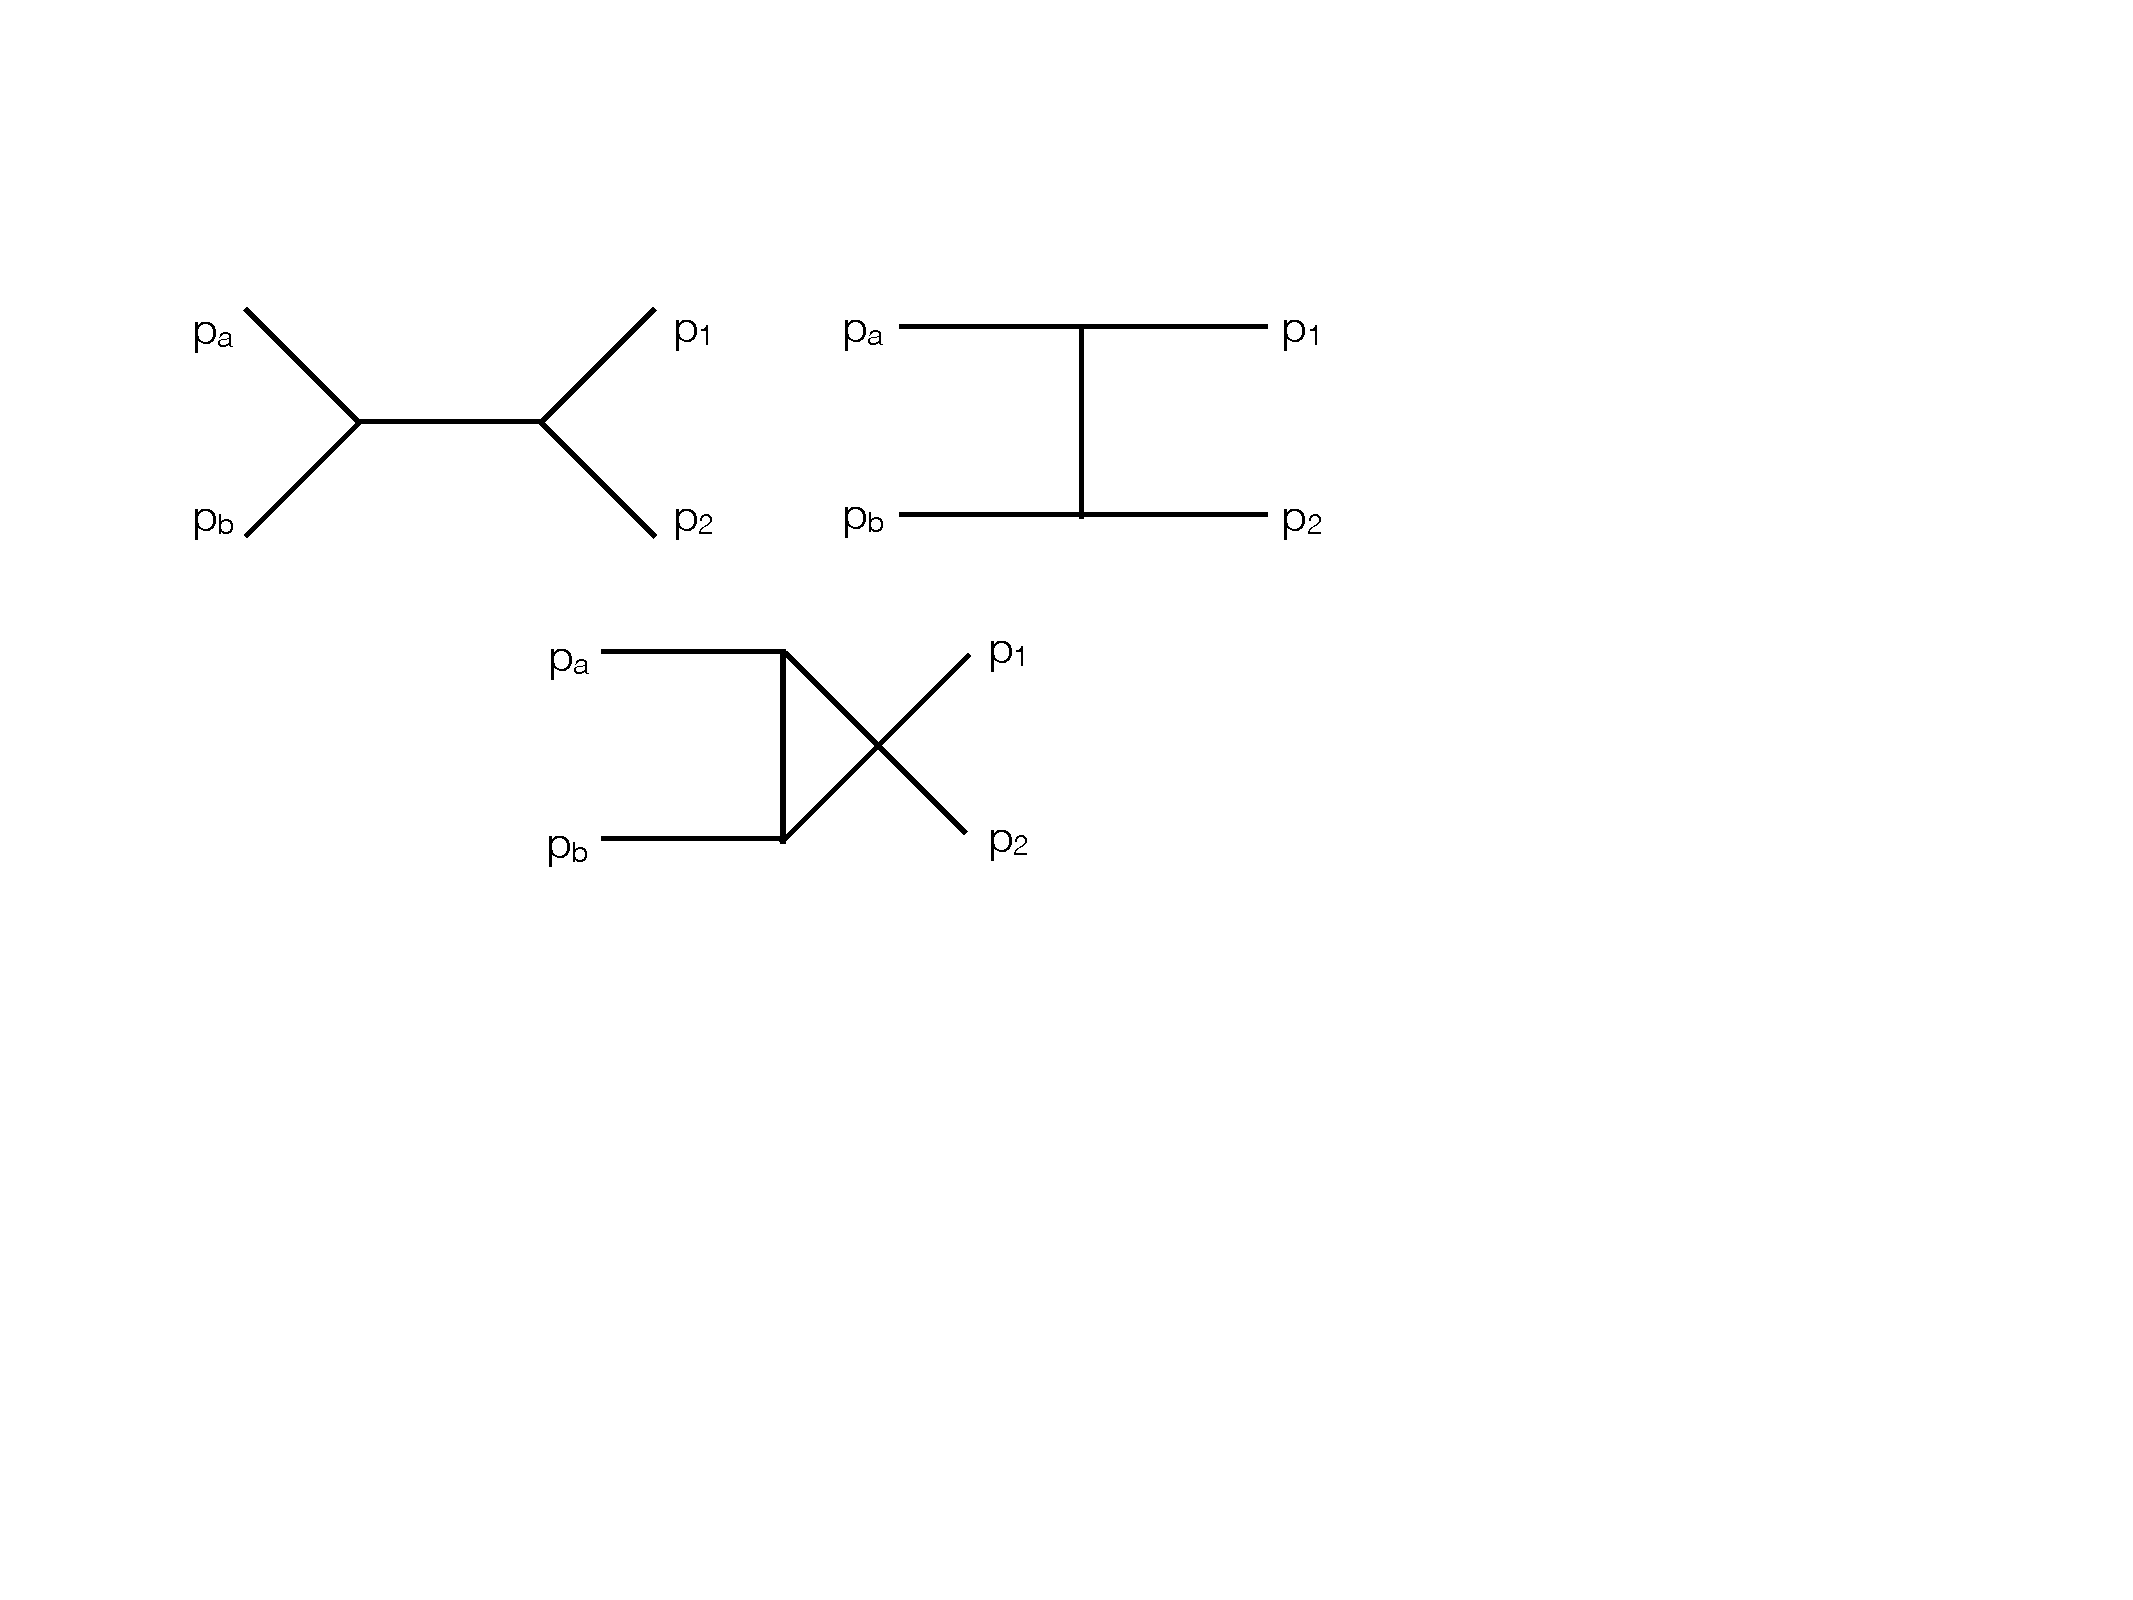
\includegraphics[scale=0.6]{Images/feyndiags.pdf} 
\caption{Example Feynman diagrams. The top-left diagram is called the $s$-channel, the top-right the $t$-channel and the bottom the $u$-channel. All momenta flow from left to right.}
\label{fig:feyndiags}
\end{figure}

The topology of these diagrams is commonly seen in many physical theories as well; they have the special names $s$-channel, $t$-channel and $u$-channel. These names come from the \emph{Mandelstam variables} which refer to the invariant mass  present in the intermediate propagator in each diagram, fixed by momentum conservation at each vertex; $s = (p_a + p_b)^2$, $t = (p_a - p_1)^2$ and $u = (p_a - p_2)^2$. \\
\\
Now that we have seen the general procedure for drawing diagrams, we need mathematical rules to convert these diagrams into calculable expressions. These are the famous \emph{Feynman rules} and while there is a general way of deriving them for any given theory we will jump straight to the rules we need for the theory of QCD that the rest of the thesis depends upon: 

\begin{enumerate}
\item{\emph{External Fermion Lines}. For an external quark, associate a factor $u(p)$ for incoming and $\bar{u}(p)$ for outgoing. For external anti-quarks, associate a factor $\bar{v}(p)$ for incoming and $v(p)$ for outgoing. To ensure consistent multiplication in the spinor indices, follow a quark line backwards through the diagram.}
\item{\emph{External Gluon Lines}.  Associate a factor $\varepsilon_\mu(p)$ for incoming and $\varepsilon^*_\mu(p)$ for outgoing. These objects are the so-called \emph{polarisation vectors} of the gluons and arise from solving their equations of motion.}
\item{\emph{Internal propagators}. For each internal propagator, associate the relevant factor as detailed in table \ref{tab:QCD}.}
\item{\emph{Vertices}. For each vertex, associate the relevant factor as detailed in table \ref{tab:QCD}.}
\item{\emph{Unconstrained momentum}. Beyond first order in perturbation theory, Feynman graphs will contain momenta that are not fixed by momentum conservation, resulting in what are called \emph{loops}. For each such momenta $k$, include an integration $\int \frac{d^4 k}{(2 \pi)^4}$. }
\item{\emph{Extra signs}. Each fermion or anti-fermion loop comes with a factor of (-1) and each anti-fermion line that flows from the initial state to the final state also comes with a factor of (-1). These rules result from the fact the fermion operators anti-commute; an explicit demonstration of precisely why we need these extra considerations will not be shown.}
\end{enumerate}

Following these rules and adding together all diagrams results in the quantity $i M$, where $M$ is the \emph{matrix element} or \emph{amplitude} $\left<f | i \right>$ at the calculated order in the coupling expansion. Later on, we will see exactly how this relates to a physical quantity. 

\begin{table}[h!]
  \centering
  \begin{tabular}{ | c | m{5cm} | m{5cm} | }
    \hline
    Diagrammatic Element & Description & Feynman Rule \\ \hline
    \begin{minipage}{.3\textwidth}
      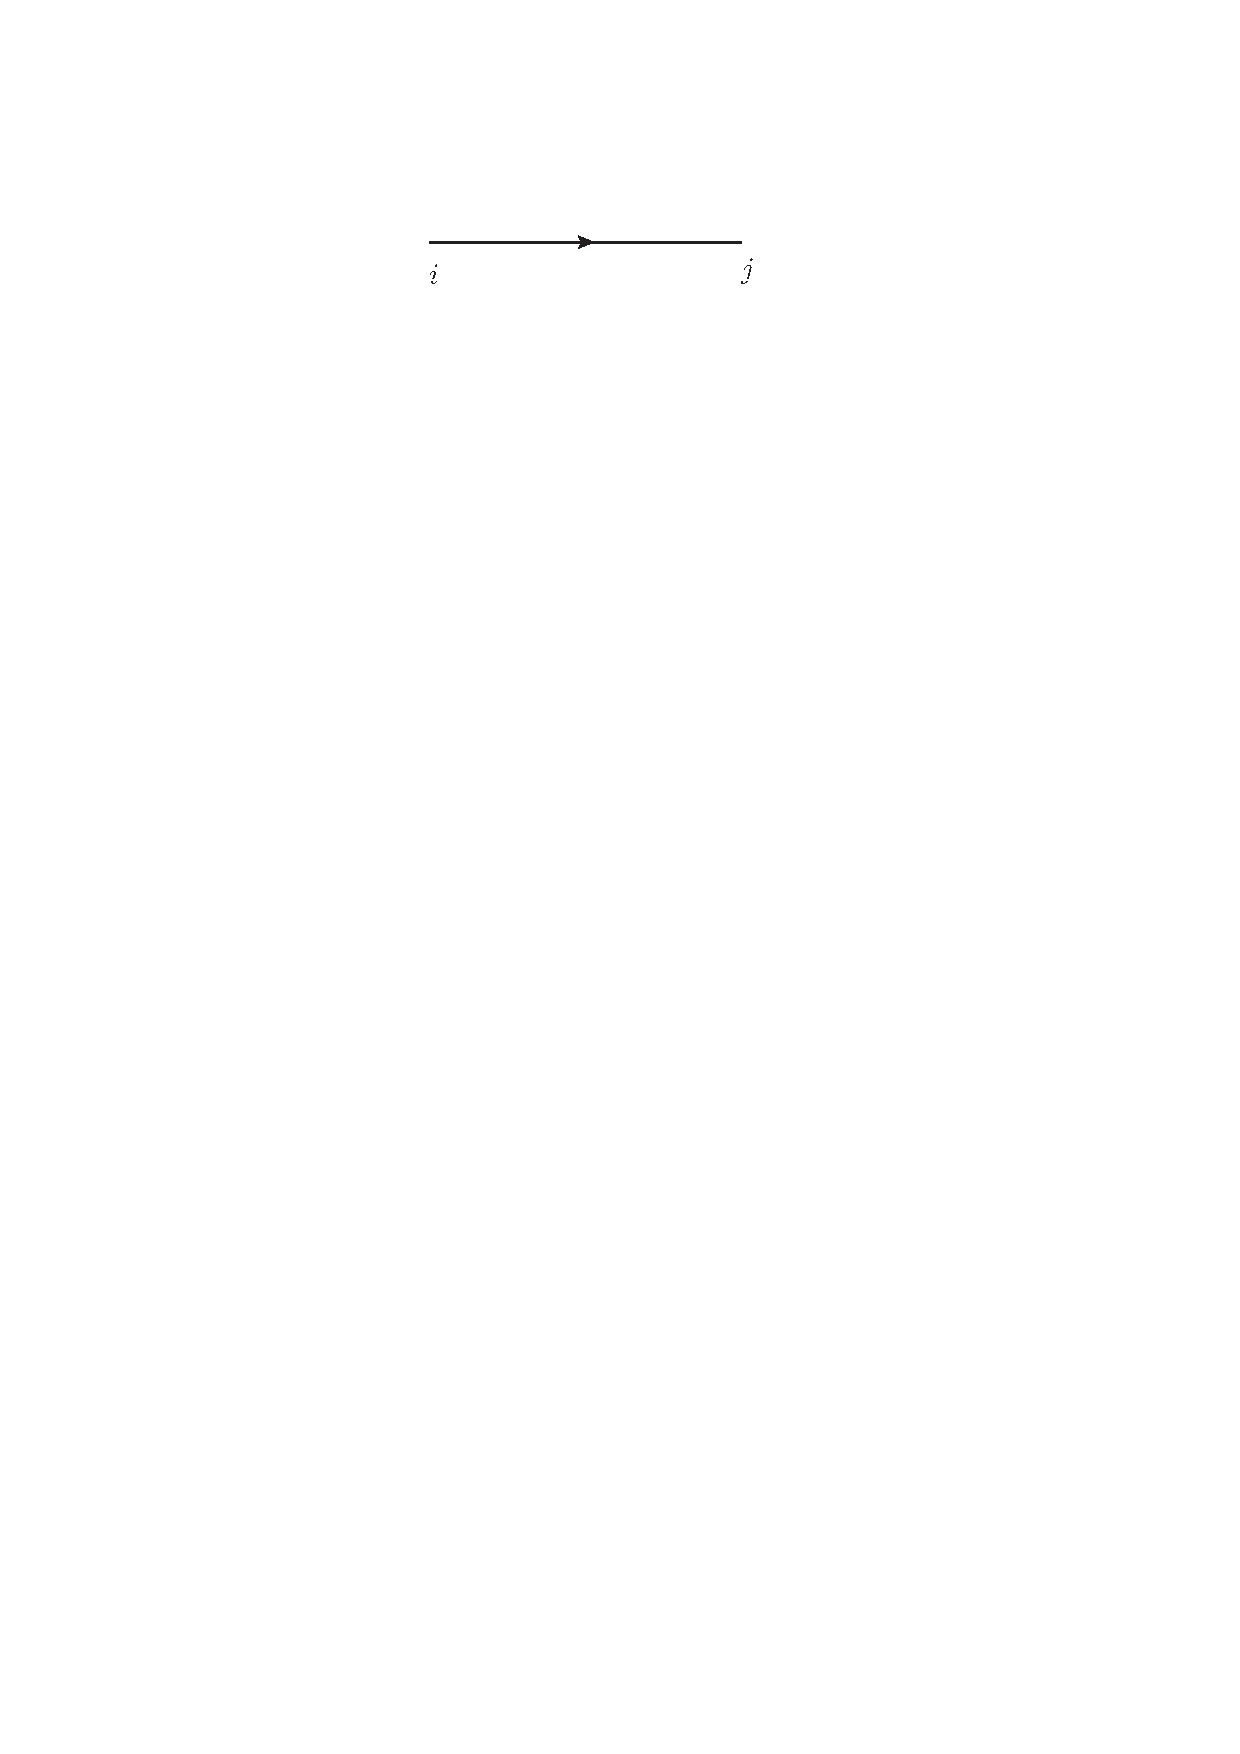
\includegraphics[scale=0.7]{Images/ferm_prop.pdf}
      \\
    \end{minipage}
    &
    \begin{minipage}[t]{5cm}
    Quark Propagator with fundamental colour index $i \to j$, momentum $p$ and mass $m_f$
    \end{minipage}
    & 
    \begin{minipage}{5cm}
    \centering
     $$\frac{i \delta_{ij}}{\slashed{p} - m_f} = \frac{i \delta_{ij} (\slashed{p}+m_f)}{p^2-m_f^2}$$
    \end{minipage}
    \\ [\VSpace]
	\begin{minipage}{.3\textwidth}
      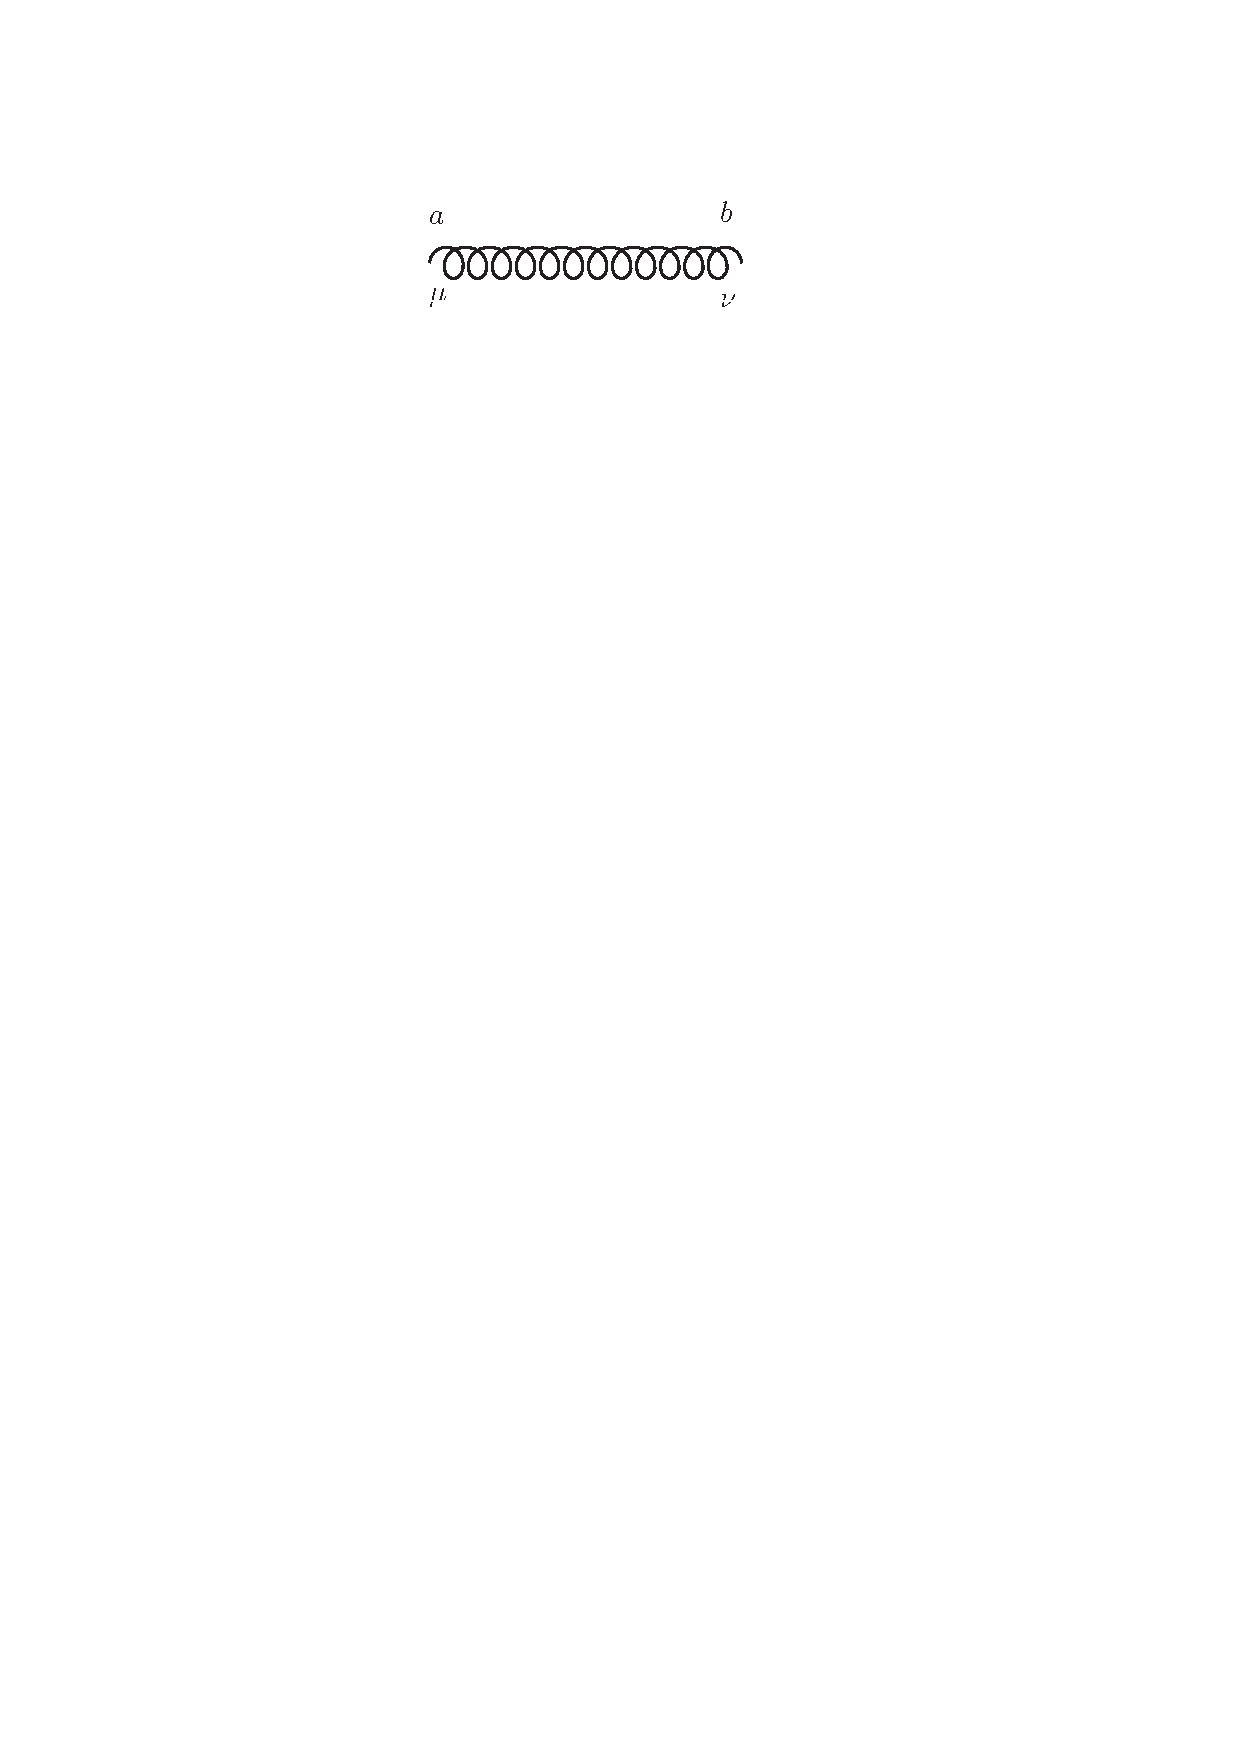
\includegraphics[scale=0.7]{Images/gluon_prop.pdf}
    \end{minipage}
    &
    %\begin{minipage}[t]{5cm}
    Gluon Propagator with adjoint colour index $a \to b$ and momentum $p$
    %\end{minipage}
    & 
    \begin{minipage}{5cm}
    \centering
     $$\frac{-i \delta^{ab} \eta^{\mu \nu}}{p^2}$$
    \end{minipage}
    \\ [\VSpace]
    	\begin{minipage}{.3\textwidth}
      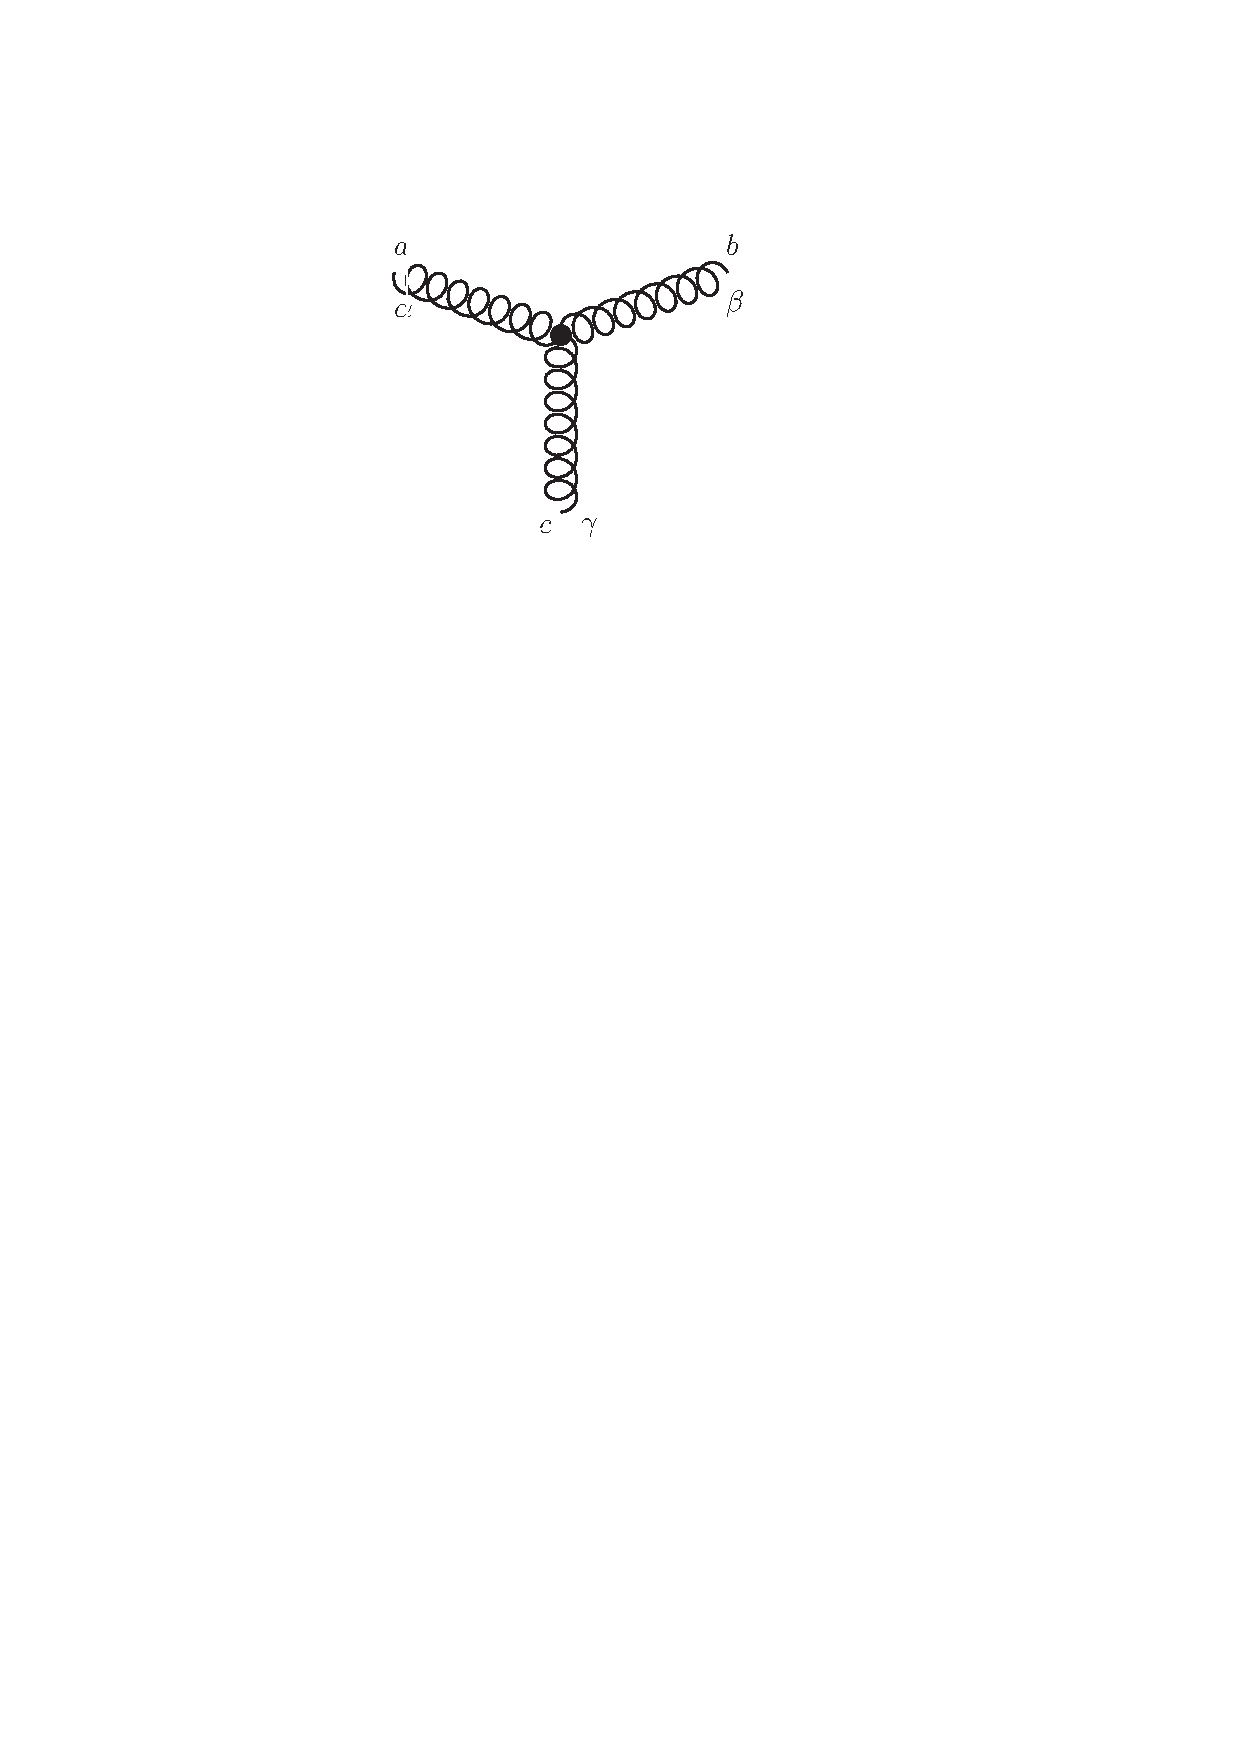
\includegraphics[scale=0.7]{Images/3g_vert.pdf}
    \end{minipage}
    &
    %\begin{minipage}[t]{5cm}
    Three-Gluon Vertex. All momenta taken as incoming, with $k_1$ associated with the gluon with adjoint index $a$, $k_2$ with $b$ and $k_3$ with c
    %\end{minipage}
    & 
    \begin{minipage}{5cm}
    \centering
     $ -g_s f^{abc} ( \eta^{\alpha \beta}(k_1 - k_2)^\gamma
     + \eta^{\beta \gamma}(k_2 -k _3)^\alpha
     + \eta^{\gamma \alpha}(k_3 - k_1)^\beta ) $
    \end{minipage}
    \\ [\VSpace]
        	\begin{minipage}{.3\textwidth}
      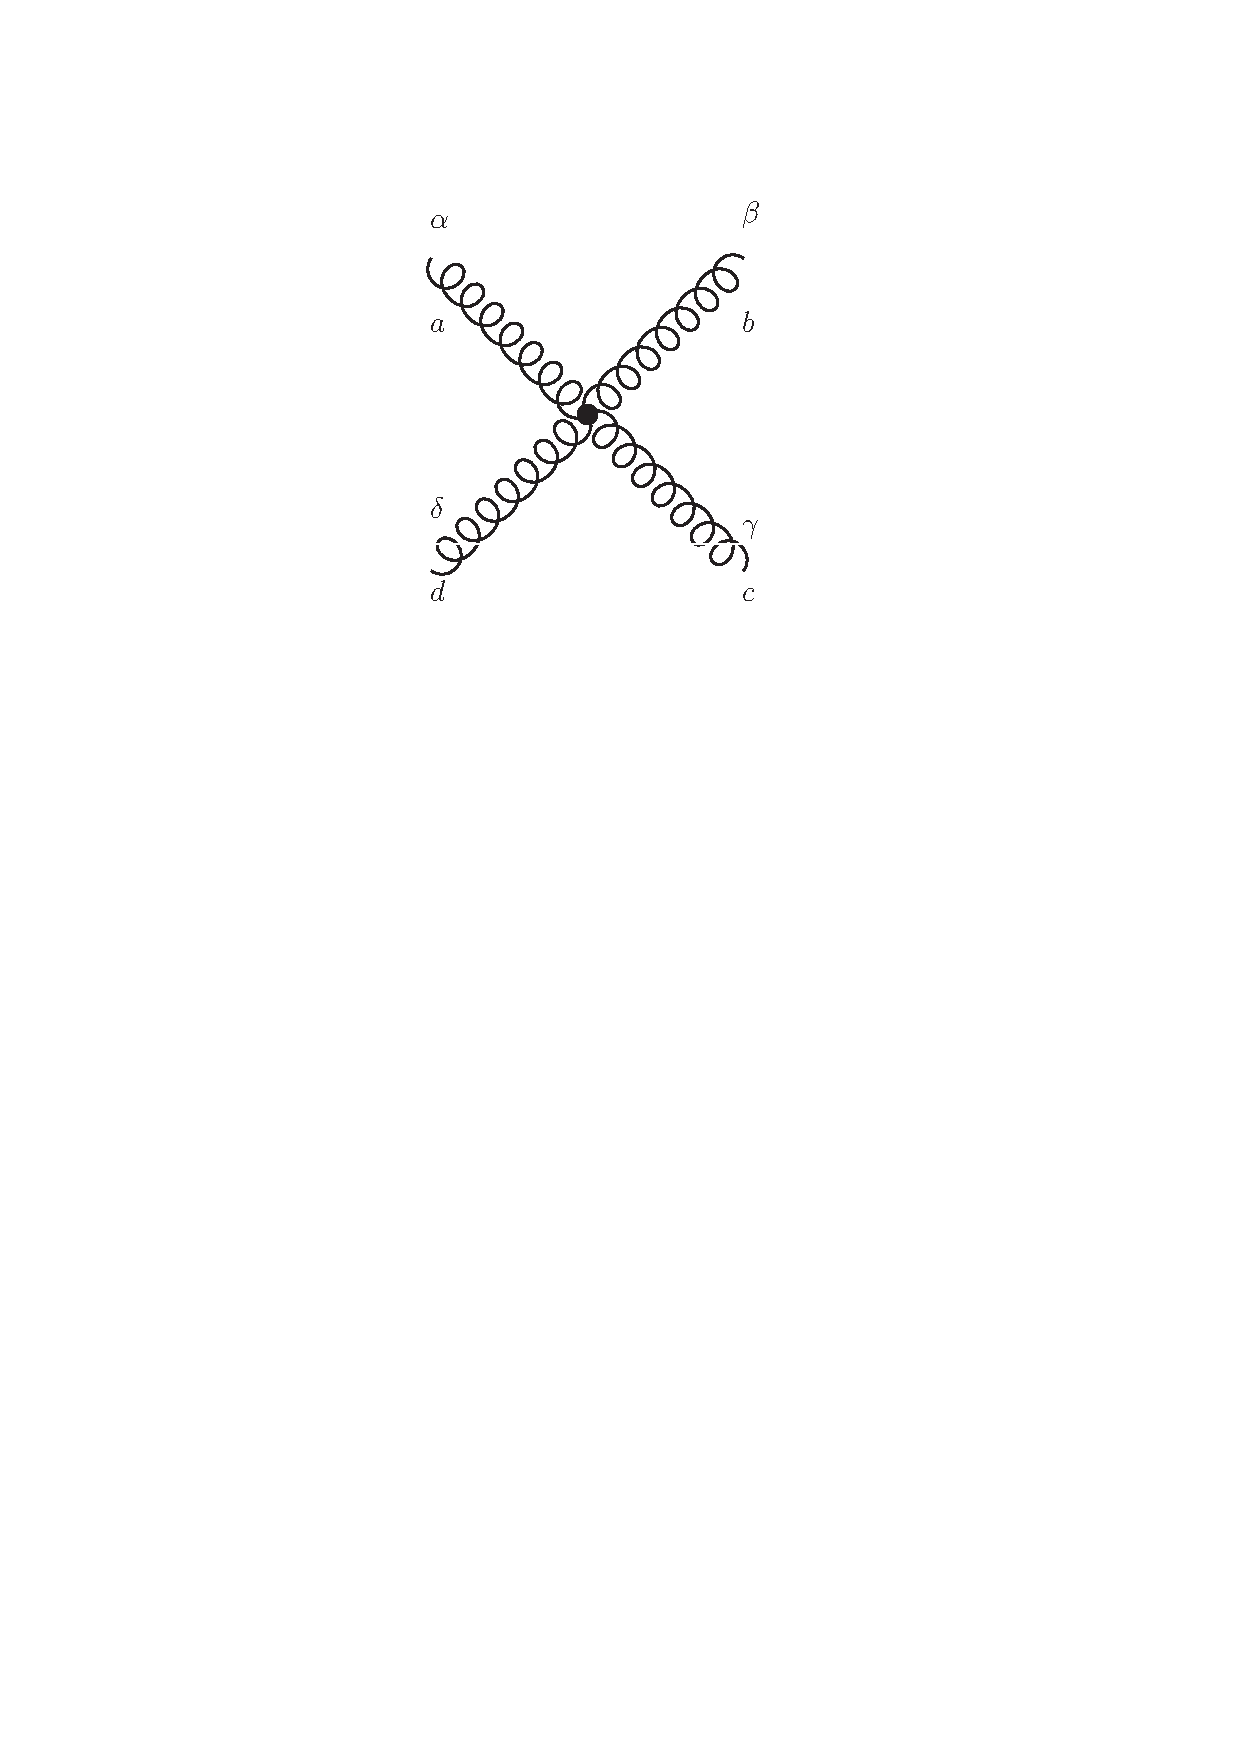
\includegraphics[scale=0.7]{Images/4g_vert.pdf}
    \end{minipage}
    &
    %\begin{minipage}[t]{5cm}
    Four-Gluon Vertex with adjoint indices $a,b,c,d$
    %\end{minipage}
    & 
    \begin{minipage}{5cm}
    \centering
     $  -ig_s^2 (f^{ade}f^{cde}(\eta^{\alpha \gamma} \eta^{\beta \delta} - \eta^{\alpha \delta} \eta^{\beta \gamma}) + f^{ace}f^{bde}(\eta^{\alpha \beta} \eta^{\gamma \delta} - \eta^{\alpha \delta} \eta^{\gamma \beta}) + f^{ade}f^{bce}(\eta^{\alpha \beta} \eta^{ \delta \gamma } - \eta^{\alpha \gamma} \eta^{\delta \beta}))$
    \end{minipage}
    \\ [\VSpace]
            	\begin{minipage}{.3\textwidth}
      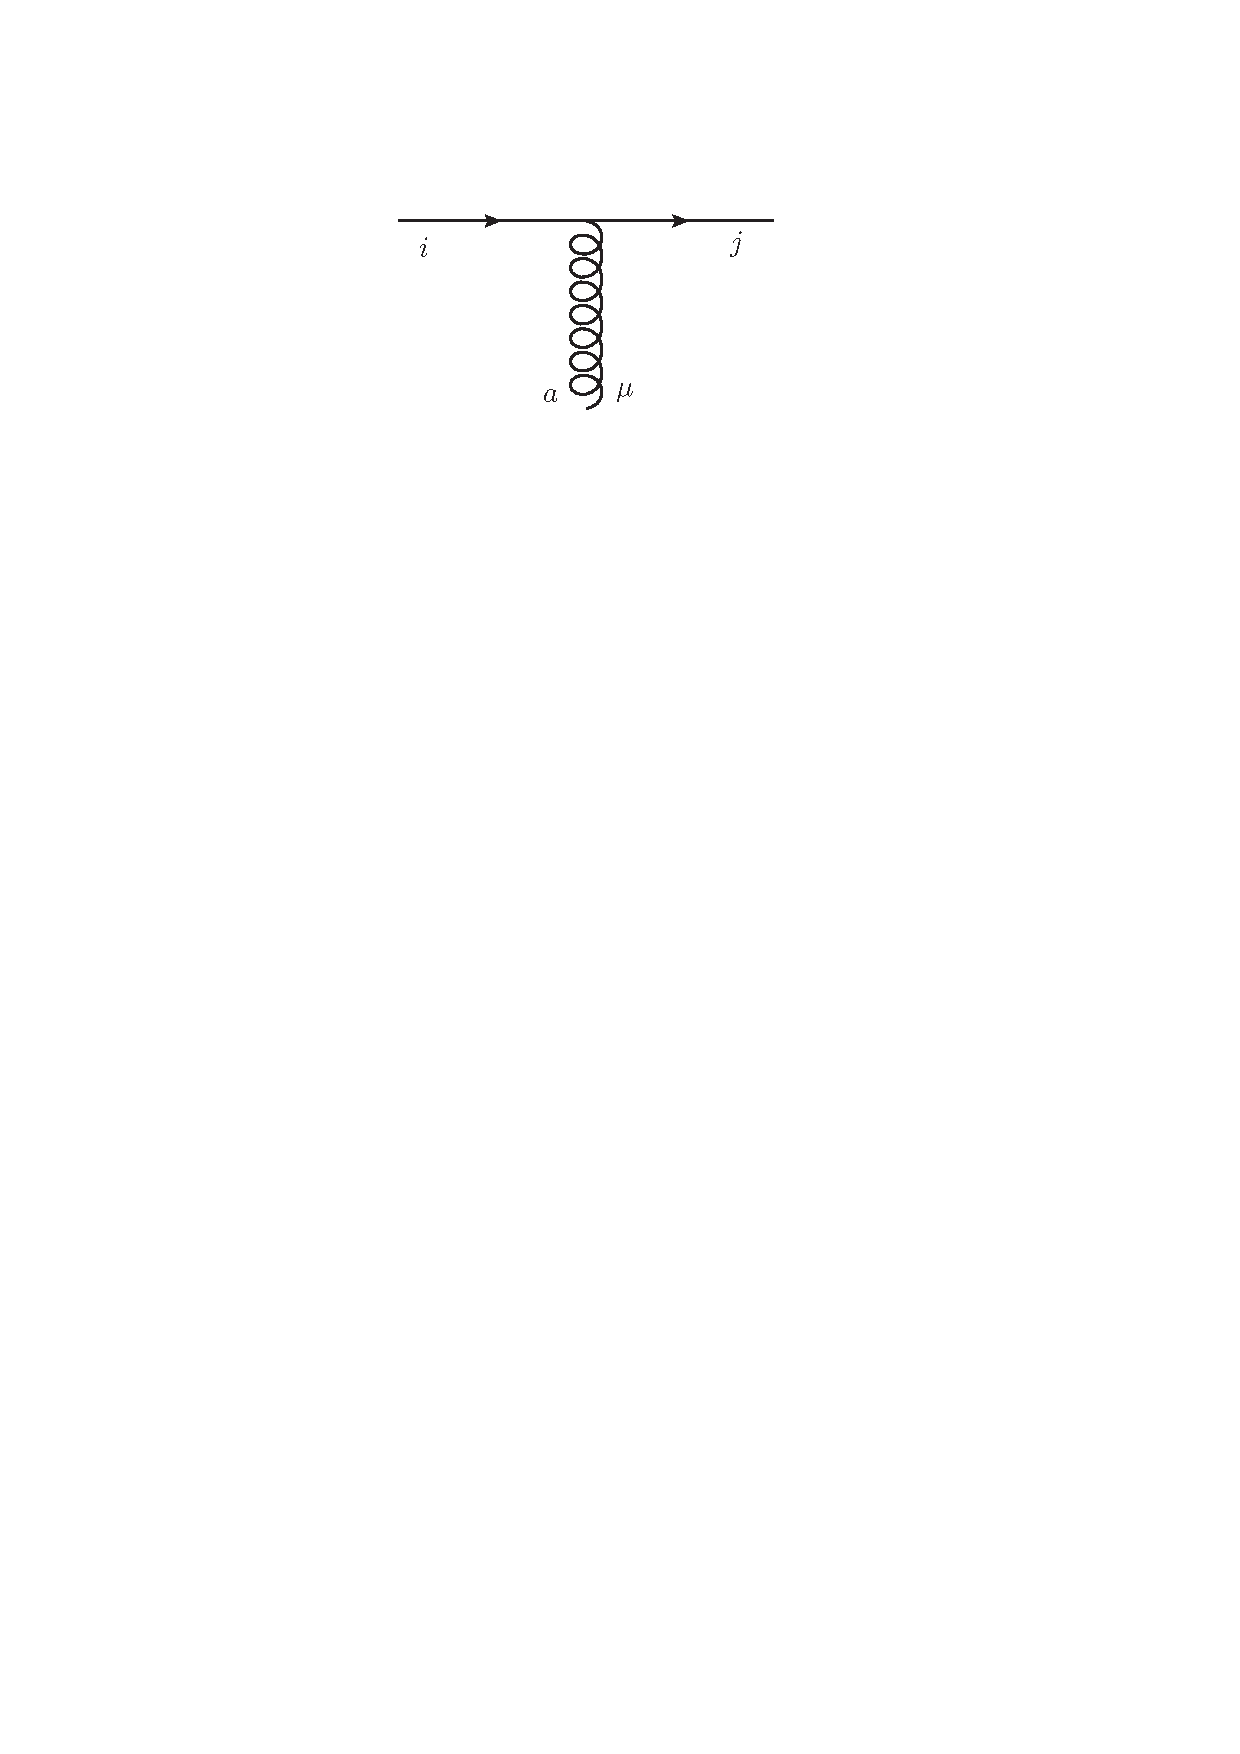
\includegraphics[scale=0.7]{Images/qg_vert.pdf}
    \end{minipage}
    \hspace{2pt}
    &
    %\begin{minipage}[t]{5cm}
    Quark-Gluon Vertex with fundamental indices $i,j$ and adjoint index $a$
    %\end{minipage}
    & 
    \begin{minipage}{5cm}
    \centering
     $$  -i g_s \gamma^\mu t^a_{ij}$$
    \end{minipage}
    \\ [\VSpace]

    \hline
  \end{tabular}
  \caption{QCD Feynman Rules for propagators and vertices}\label{tab:QCD}
\end{table}

\subsection{$qQ \to qQ$ at Leading Order}
\todo{reword first sentence}
As an explicit exercise in performing QCD calculations with Feynman rules, let us take an example of an up quark scattering off a down quark into again an up quark and a down quark. This process is particularly simple because there is only one contributing Feynman diagram, shown in figure \ref{fig:qQqQ}.

\begin{figure}[t]
\centering
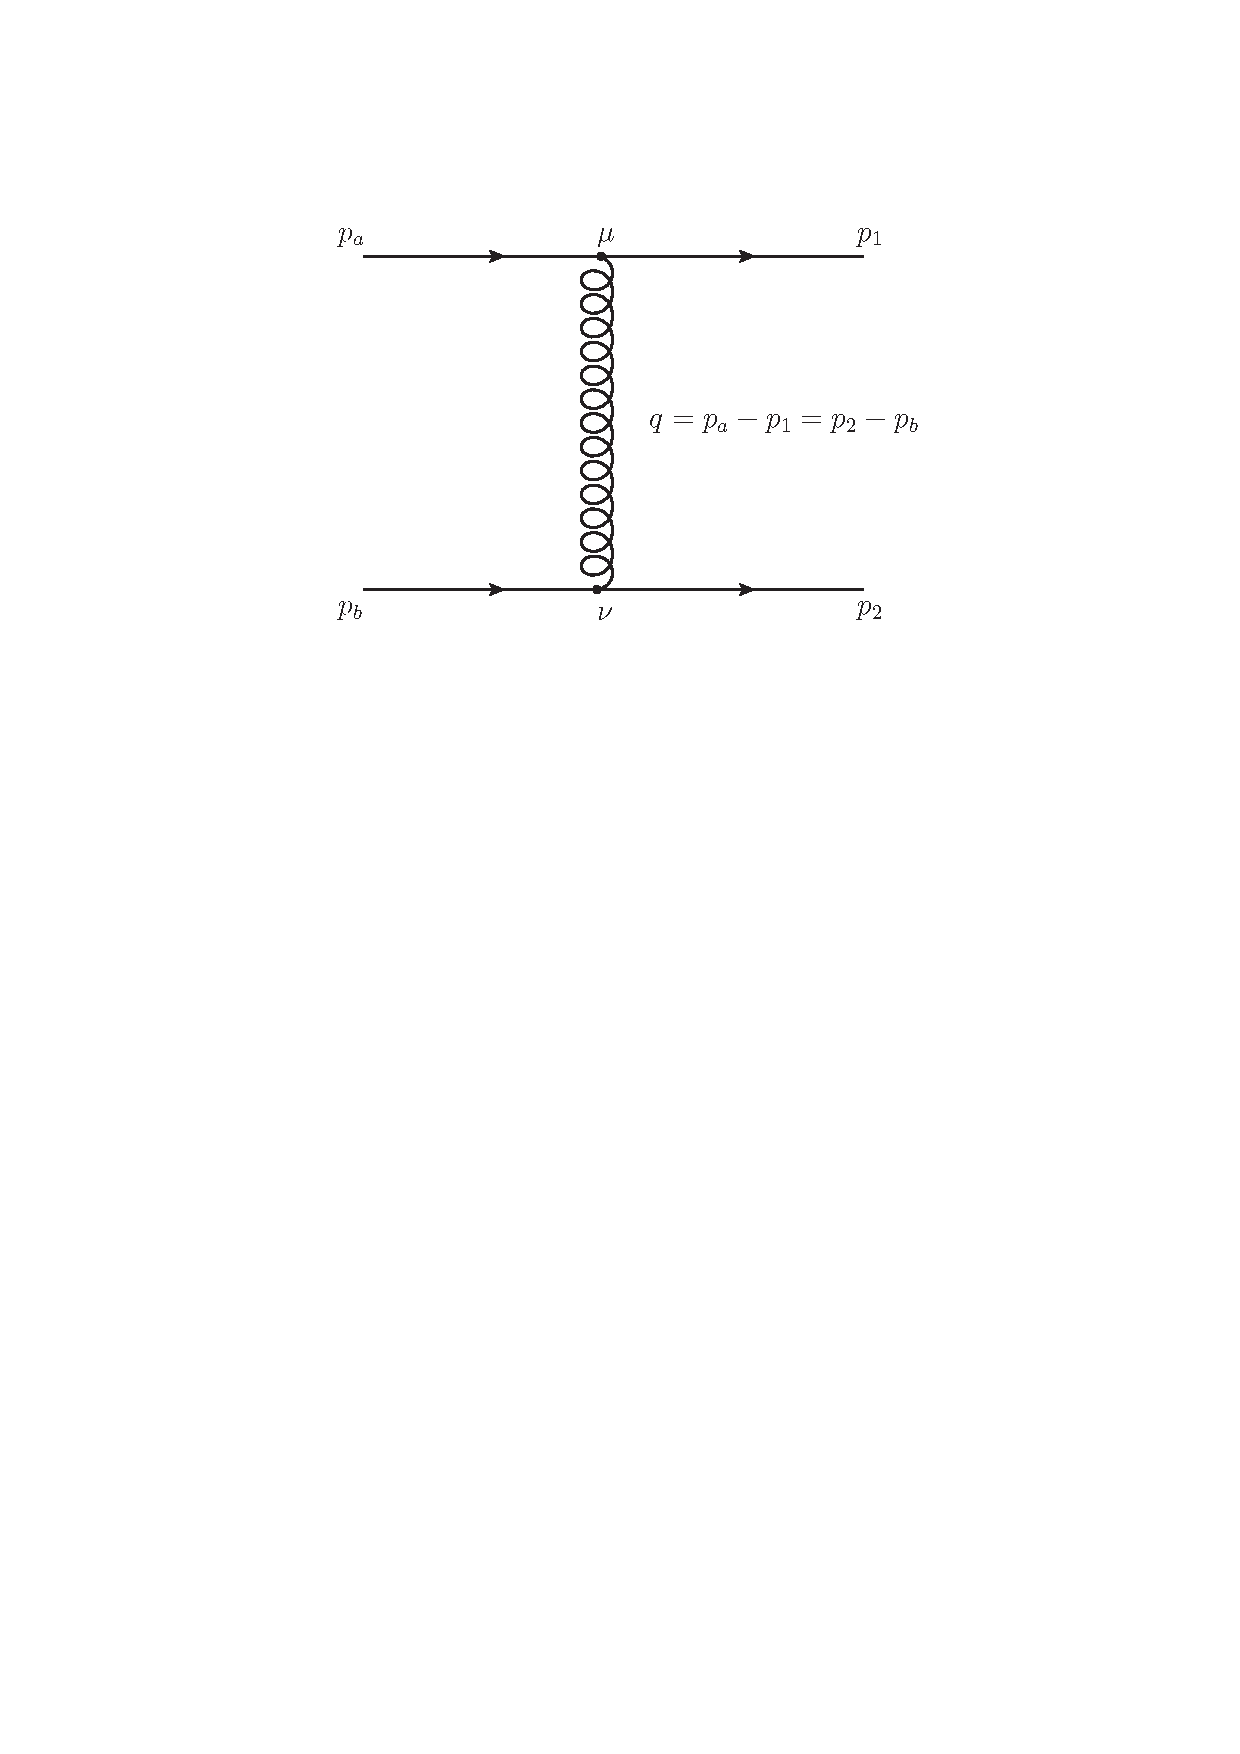
\includegraphics[scale=0.75]{Images/qQ_t.pdf} 
\caption{Two quarks of different flavour scattering via the exchange of a gluon in the $t$-channel.}
\label{fig:qQqQ}
\end{figure}

Applying the Feynman rules, we arrive at the expression for the amplitude:
\begin{equation}
\begin{split}
iM &= \bar{u}(p_2) (-i g_s t^b \gamma^\nu)u(p_b) \left(\frac{-i \eta_{\mu \nu} \delta^{ab}}{(p_a-p_1)^2} \right)\bar{u}(p_1)(-i g_s t^a \gamma^\mu) u(p_a) \\
&= \left(\frac{t^b \delta^{ab} t^a i g_s^2 }{(p_a-p_1)^2}\right) \bar{u}(p_2) \gamma_\mu u(p_b) \bar{u}(p_1)\gamma^\mu u(p_a) \\
&= \left(\frac{t^a \delta^{ab} t^b i g_s^2 }{\hat{t}}\right) \bar{u}(p_2) \gamma_\mu u(p_b) \bar{u}(p_1)\gamma^\mu u(p_a),
\end{split}
\end{equation}

where we have for now suppressed the colour and spin dependence of the quark spinors. In general, there is no control over the colours and spins of the particles in our experiment and so we should take this into account, by averaging over all initial state spins/colours and summing over all final state spins/colours. From the general laws of Quantum Mechanics \cite{Dirac}, we know that any physical quantity must be proportional to $|M|^2$. Since each helicity and colour configuration are physically distinguishable (that is, they do not interfere with each other quantum mechanically, we are just ignorant of what the states are), this sum/average must be done at the $|M|^2$ level: \todo{explain M notation better}

\begin{equation}
|\bar{M}|^2 = \frac{1}{9} \times \frac{1}{4} \times \frac{g_s^4}{\hat{t}^2} \times \sum_{colours}  \sum_{spins} |\tilde{M}|^2,
\end{equation}

where we have stripped some factors that don't depend on the spins/colours out of the matrix elements. We will begin by performing the spin sum. It will be useful to keep track of spinor indices in this calculation, which are implicitly summed over, and introduce the notation $u(p) \equiv u_p$ to get

\begin{equation}
\begin{split}
\sum_{spins}|\tilde{M}|^2 &= \sum_{spins}  [\bar{u}_2^{i_1} \gamma_\mu^{i_1 j_1} u_b^{j_1}][\bar{u}_1^{i_2}\gamma^{\mu, i_2 j_2} u_a^{j_2}] [\bar{u}_2^{i_3}\gamma_\nu^{i_3 j_3} u_b^{j_3}]^\dagger [\bar{u}_1^{i_4}\gamma^{\nu, i_4 j_4} u_a^{j_4}]^\dagger \\
&= \sum_{spins}  [\bar{u}_2^{i_1} \gamma_\mu^{i_1 j_1} u_b^{j_1}][\bar{u}_1^{i_2}\gamma^{\mu, i_2 j_2} u_a^{j_2}] [\bar{u}_b^{i_3} \gamma_\nu^{i_3 j_3}  u_2^{j_3}][\bar{u}_a^{i_4}  \gamma^{\nu, i_4 j_4} u_1^{j_4}],
\end{split}
\end{equation}

where we have used $(\gamma^0)^\dagger = \gamma^0$ and $(\gamma^\mu)^\dagger = \gamma^0 \gamma^\mu \gamma^0$. At this point we introduce the important result

\begin{equation}
\sum_{spins} u_p \bar{u}_p = \slashed{p} + m, 
\end{equation}

which amounts to the statement that the set of $u$ functions is complete and, for simplicity, we will take the mass of the quarks in our calculation to be zero. This is a good approximation if the momenta of the particles involved in the scattering are much larger than the value of the mass. We will always assume this is the case unless otherwise stated in the entirety of this thesis. Using this result to rewrite our amplitude and being careful with spinor indices, we see

\begin{equation}
\begin{split}
\sum_{spins}|\tilde{M}|^2  & =  [\slashed{p}_b^{j_1 i_3} \gamma_\nu^{i_3 j_3} \slashed{p}_2^{j_3 i_1} \gamma_\mu^{i_1 j_1}][\slashed{p}_a^{j_2 i_4} \gamma^{\nu,i_4 j_4} \slashed{p}_1^{j_4 i_2} \gamma^{\mu,i_2 j_2}] \\
&= Tr[\gamma_\alpha \gamma_\nu \gamma_\beta \gamma_\mu]p_b^\alpha p_2^\beta \times Tr[\gamma^\rho \gamma^\nu \gamma^\sigma \gamma^\mu] p_{a, \rho} p_{1, \sigma}.
\end{split}
\end{equation}

What remains is to evaluate the traces of the products of gamma matrices. There are a whole host of so-called \emph{trace theorems} \cite{Peskin1995}, of which we quote one result:\footnote{This result only applies in a 4-dimensional spacetime, which we have in this problem, but can be generalised to $D$ dimensions if required.}

\begin{equation}
Tr[\gamma^\alpha \gamma^\nu \gamma^\beta \gamma^\mu] = 4(\eta^{\alpha \nu} \eta^{\beta \mu} - \eta^{\alpha \beta} \eta^{\nu \mu} + \eta^{\alpha \mu} \eta^{\nu \beta}).
\end{equation}

Applying this result to our calculation, we arrive at
\begin{equation}
\begin{split}
\sum_{spins}|\tilde{M}|^2 &= 16 (p_{b, \nu} p_{2, \mu} - p_b \cdot p_2 \eta_{\nu \mu} + p_{b, \mu} p_{2, \nu}) \times (p_a^\nu p_1^\mu - p_a \cdot p_1 \eta^{\nu \mu} + p_a^\mu p_1^\nu) \\
&= 32 \left((p_b \cdot p_a)(p_1 \cdot p_2) + (p_b \cdot p_1)(p_2 \cdot p_a) \right),
\end{split}
\end{equation}

which is a simple result. The final ingredient of the amplitude is the colour sum. Since this is the first time we are performing such a calculation, it is instructive to do this in detail. We write out the colour indices in full \cite{Skands2011}:

\begin{equation}
\begin{split}
\sum_{colours} |\tilde{M}|^2 & \sim \sum_{colours} [t^a_{q_1, q_a} \delta^{ab} t^b_{q_2, q_b}] [t^c_{q_1,q_a} \delta^{cd} t^d_{q_2, q_b}]^\dagger \\
&= \sum_{a,b,c,d,q_1,q_a,q_2,q_b} [t^a_{q_1, q_a} \delta^{ab} t^b_{q_2, q_b}] [t^c_{q_a,q_1} \delta^{cd} t^d_{q_b, q_2}] \\
&= \sum_{a,c,q_1,q_a,q_2,q_b} [t^a_{q_1, q_a} t^a_{q_2, q_b}] [t^c_{q_a,q_1} t^c_{q_b, q_2}] \\
&= \sum_{a,c} Tr(t^a t^c) Tr(t^a t^c) \\
&= \sum_{a,c} \frac{1}{2} \delta^{ac} \frac{1}{2} \delta^{ac} \\
&= \sum_a \frac{1}{4} \delta^{aa} \\
&= 2.
\end{split}
\end{equation}

Combining the results, we find an expression for the full amplitude:

\begin{equation}
\begin{split}
|M|^2 &= \frac{16 g_s^4}{9 \hat{t}^2} \left((p_b \cdot p_a)(p_1 \cdot p_2) + (p_b \cdot p_1)(p_2 \cdot p_a) \right) \\
&= g_s^4 \times \frac{4}{9} \left(\frac{\hat{s}^2 + \hat{u}^2}{\hat{t}^2} \right).
\end{split}
\label{eqn:qQ_qQ_LO}
\end{equation}

As a matter of interest, this result is the same as the one we would get from electron-muon scattering, except with a different coupling strength and the overall factor from the colour considerations. We should expect this because our process did not involve any parts where the gluon interacts with itself and so behaves similarly to a photon in this interaction. If we were to do a next-to-leading order calculation, however, this would no longer be true and QCD loop calculations are, in general, difficult to compute.

\section{Cross-Sections in Proton-Proton Collisions}

In a collider experiment, the physical quantity is the \emph{cross section}, not the squared matrix element itself. The two are intimately related, however, by \emph{Fermi's Golden Rule}, which in this case states

\begin{equation}
d \hat{\sigma} = S \times \frac{|M|^2}{F} \times (2 \pi)^4 \delta^{(4)}(p_a + p_b - \sum_{f=1}^n p_f) \times \prod_{i=1}^n \frac{d^3 \vec{p}_i}{2 E_i (2 \pi)^3}.
\end{equation}

$|M|^2$ is the matrix element squared for the process of interest and contains all the dynamical information. $F = 4 \sqrt{(p_a \cdot p_b)^2 - m_a m_b}$  is a factor that accounts for the flux of incoming particles. The delta function ensures momentum conservation in the process. The remaining integrals are \emph{phase space} integrals over the final particles and, finally, $S$ is a statistical factor that serves to avoid over-counting in processes with indistinguishable outgoing particles -- for each group of $s$ identical particles in the final state, $S$ gains a factor $1/s!$. In theory, then, we can insert any matrix element calculated at a certain order in our perturbation theory and perform the phase space integrals to yield the cross section for any process we desire. In practice, this is not as simple as it sounds. For instance, as the number of final state particles increases, an analytic integration over their momenta becomes more and more difficult (the matrix elements as well become more difficult to compute -- a point we will revisit later). Furthermore, in QCD we cannot collide two quarks together with a well-defined energy, as our matrix element calculation might suggest, because of a property called \emph{confinement} -- because of how the strong force interacts, it is impossible to observe a free quark or gluon\footnote{Though confinement has been phenomenologically established, it is not understood from a purely theoretical viewpoint. This is essentially because it would involve calculating without the use of perturbation theory, which is a very tough task. It is therefore an outstanding problem set by the Clay Mathematics Institute to prove confinement.}. Instead, we have to collide hadrons together (for the LHC, specifically protons) which are a dynamic soup of quarks, anti-quarks and gluons (from here on, \emph{partons}). However, if the energy of the collider is large enough (which it certainly is in the LHC) then we can model a proton-proton collision as a collision of two partons within each of the protons, each of which carry some fraction of the total proton momentum. This treatment is essentially a probabilistic one and has led to the development of \emph{Parton Distribution Functions} (PDFs) \cite{Soper1997} which in itself is an area of intense research. For our purposes though, we need not discuss in detail the field of PDFs and instead just use the property that we can write our total proton-proton cross section as some convolution

\begin{equation}
d \sigma_{pp} = \sum_{f_a, f_b} \int_0^1 dx_a \int_0^1 dx_b f_a(x_a) f_b(x_b) \times d\hat{\sigma}_{partonic},
\end{equation}

where we interpret $x_a, x_b$ as the fraction of the total momentum carried by the parton from each of the protons and $f_a (x_a), f_b(x_b)$ as the value of the PDF for a parton of flavour $a,b$ carrying a momentum fraction $x_a, x_b$. This current formula does not explain all the necessary considerations, however. For example, we should expect that the form of the distribution functions has some dependence on the energy scale of the scattering, which we will call $Q^2$. The reason for this is that, as $Q^2$ is increased, one is able to probe the interior of the proton more and more precisely and thus the likelihood of picking out a certain parton of a certain momentum will depend on this scale. An example is shown in figure \ref{fig:PDF} where the behaviour of the PDF with respect to $x$ is clearly different depending on the scale. A better equation would then be

\begin{figure}[t]
\centering
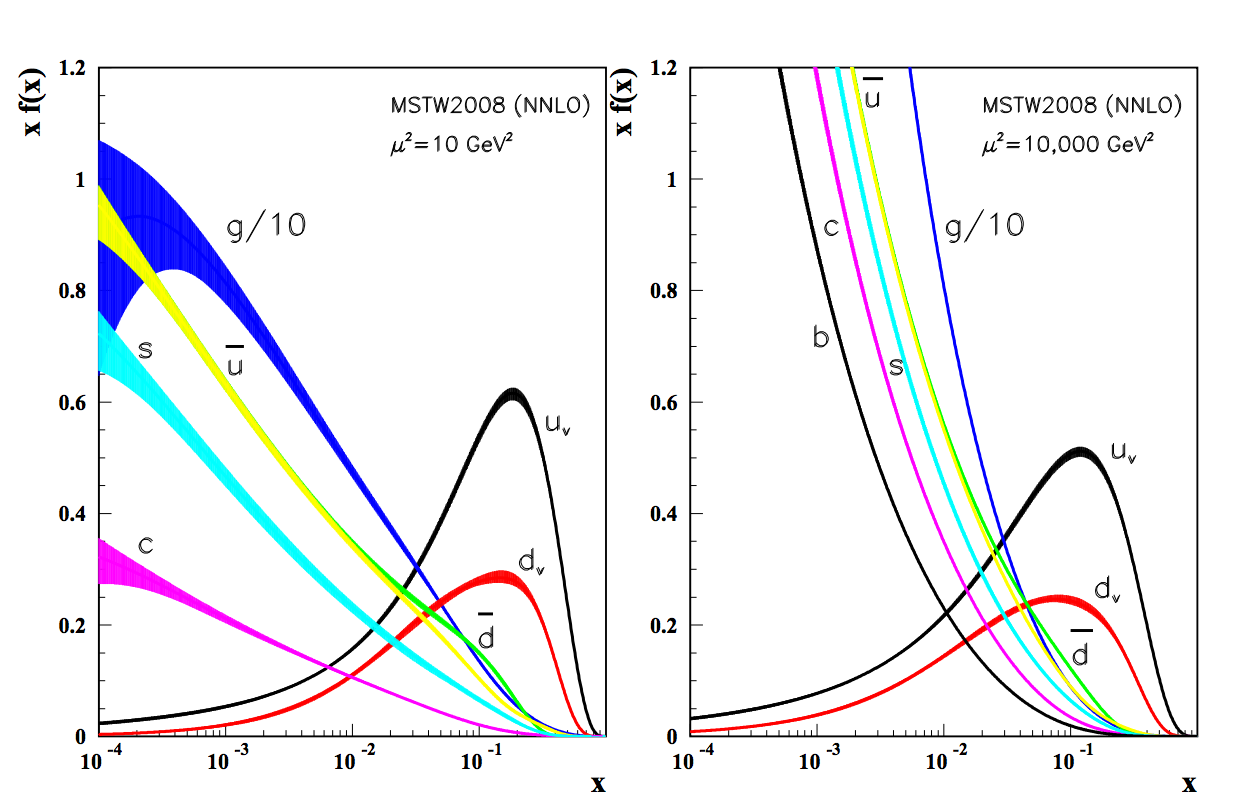
\includegraphics[scale=0.7]{Images/PDF.png} 
\caption{An example of a PDF set and how the value of the PDF changes depending on the scale probed. Figure from a review by the PDG \cite{PDG}}
\label{fig:PDF}
\end{figure}

\begin{equation}
d \sigma_{pp} = \sum_{f_a, f_b} \int_0^1 dx_a \int_0^1 dx_b f_a(x_a, Q^2) f_b(x_b, Q^2) \times d\hat{\sigma}_{partonic},
\end{equation}

for some value of $Q^2$. What that value should be, however, is somewhat mysterious -- given a hard scattering, what is the relevant scale at which the PDF is probed? This ambiguity leads to the calculation of \emph{scale variations}, which we will return to in a later chapter. Before that, we must also consider how confinement affects the final state of our scattering. The partonic cross section would lead us to believe that there are free partons after the scattering that we could detect, which goes against the principle of confinement. Indeed, we observe that the final state of partonic scatterings consists of objects called \emph{jets}, which are `cones' of hadrons and other particles caused by the \emph{hadronisation} of the partons produced in a scattering. A further discussion of the difference between partons and jets will also be discussed in a later chapter\todo{which chapter?}, but let us for now consider some `n-jet function' that `passes' an event (i.e. has value equal to 1) if there are $n$ jets present in the final state and `fails' (has value 0) otherwise. Such a function is called an \emph{exclusive} function, because only events with exactly $n$ jets will contribute, but we could also imagine an \emph{inclusive} function that will `pass' events with at least $n$ jets. We could therefore write

\begin{equation}
d \sigma_{pp \to n-jet}^{inc/exc} = \sum_{f_a, f_b} \int_0^1 dx_a \int_0^1 dx_b f_a(x_a, Q^2) f_b(x_b, Q^2) \times d\hat{\sigma}_{partonic} \times \mathcal{J}(\text{n-jet}^{inc/exc}).
\end{equation}

Generally speaking, it is not known how many jets $n$ will be produced by a scattering leaving $m$ partons in the final state and this (along with the more fundamental question of how to even properly \emph{define} a jet) is again an area of significant research. The up-shot is that, for many reasons, the calculation of QCD cross-sections is difficult and not without ambiguity. We will later see how, despite this, we can still get physically relevant results from the theory. 

\section{Spinor Helicity}
We conclude the chapter by discussing the \emph{spinor helicity formalism} for the calculation of amplitudes. The formalism makes the expression of amplitudes involving massless particles\footnote{The formalism can also be extended to include massive particles, but this is not its primary use and we will always be working with massless entities (either effectively or exactly) in this work.} less cumbersome and we will make repeated use of it throughout the remainder of this thesis. \emph{Helicity} is the projection of a particle's spin along its momentum vector and can have two values: `negative' when the spin is anti-aligned and `positive' when it is aligned. We would clearly like to describe this projection using some operator. This can be achieved by introducing a new gamma matrix $\gamma^5 = i \gamma^0 \gamma^1 \gamma^2 \gamma^3$, which can be used to project out helicity states as follows:

\begin{subequations}
\begin{align}
u_{\pm}(p_i) &= (1 \pm \gamma^5)u(p_i) \equiv \ket{i^\pm}\\
v_{\mp}(p_i) &= (1 \pm \gamma^5)v(p_i) \equiv \ket{i^\pm}\\
\bar{u}_{\pm}(p_i) &= \bar{u}(p_i) (1 \mp \gamma^5) \equiv \bra{i^\pm}\\
\bar{v}_{\mp}(p_i) &= \bar{v}(p_i) (1 \mp \gamma^5) \equiv \bra{i^\pm}.
\end{align}
\end{subequations}

We also define the basic spinor products as

\begin{subequations}
\begin{align}
\bar{u}_-(p_i)u_+(p_j) &= \bar{v}_+(p_i)v_-(p_j) = \left<i^- | j^+ \right> \equiv \left< i j \right> \\
\bar{u}_+(p_i)u_-(p_j) &= \bar{v}_-(p_i)v_+(p_j) = \left<i^+ | j^- \right> \equiv \left[ i j \right].
\end{align}
\end{subequations}

The final object we will need to deal with is a \emph{current} with the form $\bar{u} \gamma^\mu u$. Because $\gamma^5$ anti-commutes with the other gamma matrices, only currents where the two spinors have the same helicity are non-zero:

\begin{equation}
\bar{u}_{\pm}(p_i) \gamma^\mu u_{\pm}(p_j) = \matel{i^\pm}{\mu}{j^\pm} \equiv J_{ij}^{\pm, \mu}.
\end{equation}

There are many identities that these objects satisfy \cite{Dixon1996} and we list here a select few that we will use repeatedly in our calculations:

\begin{subequations}
\begin{align}
\left<i j \right> &= - \left<j i \right> \\
[i j] &= - [ji] \\
\left< i j \right>^* &= [j i ] \\
\matel{i^+}{\mu}{j^+}^\dagger &= \matel{j^+}{\mu}{i^+} \\
\matel{i^\pm}{\mu}{i^\pm} &= 2p_i^\mu \\
\matel{i^+}{\mu}{j^+} &= \matel{j^-}{\mu}{i^-} \\
\matel{i^+}{\mu}{j^+} \matel{k^+}{\mu}{l^+} &= 2 \left<j l \right> \left[k i \right] \\
 \left<i j \right> [ji] &= 2 p_i \cdot p_j = s_{ij} \\
\slashed{p}_i&= \left| i^+ \right> \left<i^+ \right| + \left|i^- \right> \left <i^- \right| \\
\left< i j \right> \left< k l \right> &= \left<i k \right> \left< j l \right> + \left< i l \right> \left< k j \right>.
\end{align}
\end{subequations}

Given their importance to this thesis, we devote some space here to the derivation of some of these results. The easiest way to do so is to pick an explicit representation for the spinors and gamma matrices and work in individual components. It is instructive to work in \emph{light cone coordinates} where we make the substitution $p^{\pm} = E \pm p_z$ and parametrise momenta transverse to the beam axis as $p_\perp = p_x + ip_y$. For outgoing particles with four-momentum $p$, we use
\begin{subequations}
\begin{align}
u^+(p) &= 
 \begin{pmatrix}
  \sqrt{p^+} \\
  \sqrt{p^-}\frac{p_{\perp}}{|p_{\perp}|}\\
  0 \\
  0
 \end{pmatrix}\\
 u^-(p) &= 
 \begin{pmatrix}
  0 \\
  0 \\
  \sqrt{p^-}\frac{p_{\perp}^*}{|p_{\perp}|} \\
  -\sqrt{p^+}
 \end{pmatrix}.
\end{align}
\end{subequations}
\begin{subequations}
For incoming particles with 4-momentum $p$ moving along the positive light cone direction, we use: 
\begin{align}
u^+(p) &= 
 \begin{pmatrix}
  \sqrt{p^+} \\
  0\\
  0 \\
  0
 \end{pmatrix}\\
 u^-(p) &= 
 \begin{pmatrix}
  0 \\
  0 \\
  0 \\
  -\sqrt{p^+}
 \end{pmatrix}.
\end{align}
\end{subequations}
\begin{subequations}
For incoming particles with 4-momentum $p$ moving in the negative light cone direction, we use:
\begin{align}
u^+(p) &= 
 \begin{pmatrix}
  0 \\
  -\sqrt{p^-}\\
  0 \\
  0
 \end{pmatrix}\\
 u^-(p) &= 
 \begin{pmatrix}
  0 \\
  0 \\
  -\sqrt{p^-} \\
  0
 \end{pmatrix}.
\end{align}
\end{subequations}

We also use the following representation of the gamma matrices: %\todo{remove this if I put it in Appendix}
\begin{subequations}
\begin{align}
\gamma^0 &= 
 \begin{pmatrix}
  0 & 0 & 1 & 0\\
  0 & 0 & 0 & 1\\
  1 & 0 & 0 & 0\\
  0 & 1 & 0 & 0
 \end{pmatrix}\\
 \gamma^1 &= 
 \begin{pmatrix}
  0 & 0 & 0 & -1\\
  0 & 0 & -1 & 0\\
  0 & 1 & 0 & 0\\
  1 & 0 & 0 & 0
 \end{pmatrix}\\
 \gamma^2 &= 
 \begin{pmatrix}
  0 & 0 & 0 & i\\
  0 & 0 & -i & 0\\
  0 & -i & 0 & 0\\
  i & 0 & 0 & 0
 \end{pmatrix}\\
 \gamma^3 &= 
 \begin{pmatrix}
  0 & 0 & -1 & 0\\
  0 & 0 & 0 & 1\\
  1 & 0 & 0 & 0\\
  0 & -1 & 0 & 0
 \end{pmatrix}.
 \end{align}
 \end{subequations}

With our conventions defined, we can move on to some derivations. An identity that is used often is $\matel{i^\pm}{\mu}{i^\pm} = 2p_i^\mu$ so this would be a sensible one to prove. If we have an incoming particle with momentum $p$, then the first element of the product is (we take positive helicity particles)

\begin{equation}
\matel{i^+}{0}{i^+} = (u_i^+)^\dagger \gamma^0 \gamma^0 u_i^+ =  (u_i^+)^\dagger u_i^+ = p_i^+.
\end{equation}

By inspection, we see that such a product will only be non-zero if the multiplication $\gamma^0 \gamma^\mu$ applied to $u_i^+$ is such that there is a non-zero component in the first component of the resulting spinor. In other words, the product $\gamma^0\gamma^\mu$ must have a non-zero entry in the top-left. Explicit calculation of $\gamma^0 \gamma^1$ and $\gamma^0 \gamma^2$ shows this not to be the case, and so

\begin{equation}
\matel{i^+}{1}{i^+} = \matel{i^+}{2}{i^+} = 0.
\end{equation}

Finally, the product $\gamma^0 \gamma^3$ does have a non-zero entry in the top-left which is equal to 1 and thus

\begin{equation}
\matel{i^+}{3}{i^+} = \matel{i^+}{0}{i^+} =  p_i^+.
\end{equation}

Converting $p_i^+$ to $E + p_z$ and remembering that the particle is massless and has no transverse component if it is incoming (i.e. $E = |p_z|$), then indeed we see that $\matel{i^\pm}{\mu}{i^\pm} = 2p_i^\mu$. The calculation for outgoing particles is longer because of the presence of the transverse term, but again this relationship is seen to hold. The other identity we will make particularly regular use of is $\left<i j \right> [ji] = s_{ij}$. To prove this, let us take $p_i$ to be incoming and along the positive direction and $p_j$ to be incoming and along the negative direction. Direct calculation then yields

\begin{equation}
\begin{split}
\left< i j \right> &= \bar{u}_i^- u_j^+ = \sqrt{p_i^+ p_j^-} \\
[ j i] &= \bar{u}_j^+ u_i^- = \sqrt{p_i^+ p_j^-},
\end{split}
\end{equation}

and thus $\left<i j \right> [ji] = p_i^+ p_j^- = (E_i + E_i)(E_j + E_j) = 4 E_i E_j = s_{ij}$. Again, the calculation involving outgoing particles is longer but the result still holds. 

As an actual practical demonstration of the technique, let us repeat the calculation in the previous section in this new language. We will once again sum over all spins (equivalent to summing over all helicities), but for clarity we work first with the case that all particles have positive helicity. Then

\begin{equation}
\begin{split}
iM_{++++} &= \bra{2^+}(-i g_s t^b \gamma^\nu) \ket{b^+} \left( \frac{- i \eta_{\mu \nu}\delta^{ab}}{(p_a - p_1)^2} \right)\bra{1^+} (-i g_s t^a \gamma^\mu)\ket{a^+} \\
& = \left(\frac{t^b \delta^{ab} t^a i g_s^2}{\hat{t}} \right) \matel{2^+}{\mu}{b^+} \matel{1^+}{\mu}{a^+} \\
& = \left(\frac{t^b \delta^{ab} t^a i g_s^2}{\hat{t}} \right) 2 \left<b a \right> [1 2]. 
\end{split}
\end{equation}

Since there are two helicity states for each particle, we would expect there to be $2^4 = 16$ different helicity configurations we would have to calculate. However, since the currents $J_{2b}$ and $J_{1a}$ disappear if the quark helicity is not conserved, we only have $4$ non-zero configurations. Furthermore, our relation $\matel{i^+}{\mu}{j^+} = \matel{j^-}{\mu}{i^-}$ reduces this to only two independent configurations. For example, the configuration where all particles have negative helicity is the same as the one with all positive helicity, except that we need to take the Hermitian conjugate of the currents. Once we take the absolute value squared of this quantity, this conjugation is irrelevant and so the amplitude contains no new information. Therefore, the only other matrix element we need to calculate is the one where the two incoming quarks have opposite helicities:

\begin{equation}
\begin{split}
iM_{+-+-} & =  \left(\frac{t^b \delta^{ab} t^a i g_s^2}{\hat{t}} \right) \matel{2^-}{\mu}{b^-} \matel{1^+}{\mu}{a^+} \\
&=  \left(\frac{t^b \delta^{ab} t^a i g_s^2}{\hat{t}} \right) \matel{b^+}{\mu}{2^+} \matel{1^+}{\mu}{a^+} \\
&=  \left(\frac{t^b \delta^{ab} t^a i g_s^2}{\hat{t}} \right) 2 \left<2 a \right> [1 b].
\end{split}
\end{equation}

The colour sum and average must still be performed, of course, but other than that we can simply take the modulus squared, sum and average over the helicities:

\begin{equation}
\begin{split}
|M|^2 &= \frac{1}{4} \times \frac{2}{9} \times \left(|M_{++++}|^2 + |M_{+-+-}|^2  + |M_{-+-+}|^2  + |M_{----}|^2 \right) \\
&= \frac{1}{18} \times \left(2 |M_{++++}|^2 + 2 |M_{+-+-}|^2 \right) \\
&= g_s^4 \times \frac{4}{9} \left(\frac{ \left<b a \right> [1 2] [ab] \left<2 1 \right> + \left<2 a \right> [1 b] [a2] \left<b 1 \right> }{\hat{t}^2}\right) \\
&=  g_s^4 \times \frac{4}{9} \left(\frac{s_{ab} s_{12} + s_{a2}s_{1b} }{\hat{t}^2} \right) \\
&= g_s^4 \times \frac{4}{9} \left(\frac{\hat{s}^2 + \hat{u}^2}{\hat{t}^2} \right),
\end{split}
\end{equation}

where in the last line we used momentum conservation to equate $s_{ab}$ with $s_{12}$ and $s_{a2}$ with $s_{1b}$ and then substituted in the relevant Mandelstam variable. This is, of course, the same result as before except we did not have to go through the trouble of evaluating the traces of gamma matrices, which is a procedure that can be quite error-prone. Furthermore, we have gained some physical insight into why the terms $\hat{s}$ and $\hat{u}$ appear in the numerator; the former comes from the helicity configuration where the quarks have the same helicity and the latter from the configuration where they are opposite. This simple example showed how easy the formalism is to work with and in the next chapter we will see how it is also powerful, in the sense that we will be able to use it to express matrix elements to all orders. 